\documentclass[11pt]{article}
\usepackage[margin={2cm,2cm}]{geometry}
\usepackage{multicol}
\usepackage{array}
\usepackage{float}
\usepackage{caption}
\usepackage{graphicx}
\usepackage{algorithm}
\usepackage{algpseudocode}
\usepackage{blindtext}

\newenvironment{Figure}
  {\par\medskip\noindent\minipage{\linewidth}}
  {\endminipage\par\medskip}

\graphicspath{ {/Users/joe/Documents/Masters_Project/NFL-Play-Call-Prediction-with-LSTM-Neural-Networks/paper/figs}}

\setlength{\columnsep}{1cm}

\title{NFL Play Call Prediction Using Sequential Neural Networks}

\author{Joseph W. Director  \\
	University of Colorado Denver \\
    MS Statistics
	\and 
	Joshua French \\
    University of Colorado Denver \\
    Advisor
    \and
    Steffen Borgwardt \\
    University of Colorado Denver \\
    Graduate Committee
    \and
    Florian Pfender \\
    University of Colorado Denver \\
    Graduate Committee
	}

\date{Spring 2022}


\begin{document}

    \pagenumbering{gobble}
    
    \maketitle

    \begin{abstract}
        \centering\begin{minipage}{\dimexpr\paperwidth-12cm}
        The prevalance of data analytics in professional sports has significantly increased over the last 20 years. 
        First popularized in \emph{Moneyball: The Art of Winning an Unfair Game (2003)}, the use of advanced analytics is now mainstream in the four major U.S. sports and abroad. 
        In the National Football League (NFL), millions of dollars are invested into analytics departments and data is being used to drive decision making at every level of an organization's operation. 
        These departments can leverage statistical methods to learn the opposition's tendencies, providing a substantial competitive advantage. 
        In particular, the defensive team can improve its strategy by accurately predicting the offensive team's play call (whether the play is a run or a pass). 
        To this end, many prior works have implemented machine learning algorithms for play call prediction. 
        However, none of the works encountered have treated play-by-play data as sequential. 
        In Football, the offensive team's current play call is dependent upon the sequence of plays called before; therefore, there is a time series component that a modeling strategy must account for. 
        In this work, we explore the ability of sequential deep learning models to predict NFL play calls.
        Namely, we compare the performance of Recurrent Neural Networks (RNNs) and Long Short Term Memory (LSTM) networks to baseline models (Logistic Regression and Gradient Boosted Decision Trees). 
        Using classification accuracy and ROC-AUC as metrics, we found that sequential models out-perform the baseline. 
        \end{minipage}
    \end{abstract}
    
    \pagebreak

    \tableofcontents
    \newpage
    \listoffigures
    \newpage
    \listoftables
    \newpage

    \pagenumbering{arabic}

    \begin{multicols*}{2}
    
    \section{Introduction}

        \subsection{Background}
            
            \paragraph{}
                Gameplay of NFL football is seperated into a sequence of instances called plays. 
                The two teams on either side of the ball are allowed to reposition themselves and prepare in betweeen these instances. 
                Given this nature, there is immense opportunity to strategize when the game is not in play.
                Akin to moving pieces on a chessboard, the coaching staff decides their team's best course of action by anticipating their opponent's moves.  
                For regular plays (i.e. not a kick-off, punt, or field goal attempt), there is a binary option for the type of play the offensive team can do; either a pass or a run.
                A strategic advantage is gained for the defensive team if they can accurately predict this outcome. 
                As a simplistic example, if they predict pass they can put more players in pass coverage, or put more players near the line of scrimmage if they predict run.
            
            \vspace{-10pt}

            \paragraph{}
                There are a number of indicators that can inform play call prediction. 
                Certain personnel packages (groups of players from various positions) and formations of the offensive team are more associated with either passes or runs. 
                Unfortunately, the NFL does not publicly release data containing specific personnel or formations. 
                However, there exists a general binary indicator for the formation; whether the play was from the shotgun (QB lines up a few yards back from the center) or under-center (QB lines up directly behind the center). 
                Beyond this, there is the in-game context of the current play. 
                This includes the down (how many plays can be used to gain the required distance), the distance (the amount of yards needed to gain in order to keep the ball), the score differential, the amount of time remaining, etc. 
                The conditions of these factors all incentivize the offensive team to use either a run or a pass play. 
                For example, if an offensive team is losing by a lot of points with little time remaining in the game, they are more likely to pass because they can gain more yards using less time. 
                Lastly, tendencies of the offensive team can be studied. 
                This is done by accumulating the relative frequency of passes to runs for the offensive team (pass to run ratio) as well as how successful they are at either passing or running (average yards gained per run or pass play).
            
            \vspace{-10pt}
            
            \paragraph{}
                An NFL coach combines experience and intuition to predict the play call. 
                In this work, experience is replaced by labeled data points from the entirety of a single NFL season (2019-2020), and intuition by a supervised machine learning algorithm. 
                A supervised machine learning task involves teaching a computer to learn the underlying patterns relating the response variable to the features \cite{Mehryar12}. 
                If the model can discern information about the features and response well enough, its predictions should generalize well to unseen instances. 
                A popular domain of machine learning is the field of deep learning. 
                Deep learning uses artificial neural networks (ANNs) that loosely resemble a biological brain. 
                They contain networks of individual neurons or nodes, each with its own activation signal, that is each capable of sending and receiving signals to other nodes (through weights) \cite{Haykin08}. 
                Types of deep learning algorithms vary in complexity and structure. 
                Here we examine recurrent neural networks (RNNs) and their variant, long short term memory (LSTM) networks. 
                These kinds of networks were originally designed for speech and text recognition because of their ability to learn sequential patterns \cite{Li15}. 

        \subsection{Problem Statement}
            \paragraph{}
                Prior works have approached play call prediction with machine learning, many implementing complex classification algorithms such as ensemble models and multi-layer perceptrons \cite{Patel20}.
                These methods only provide marginal performance increases from simplistic models such as logistic regression.
                This is because, as is often the case in machine learning tasks, the signal relating the response to the features is only so strong. 
                Therefore, in these cases, the choice of a complex algorithm provides small return as there is little that the added complexity can pick up on.
                Overcoming these performance limits requires rethinking how the data itself is structured.
                In prior approaches, each singular play is treated as a sample point. 
                Treating the data this way means the model isn't aware of any sequential patterns that may exist.
                In the approach proposed by this work, an individual sample point is represented by a play sequence of length $k$. 
        
        \end{multicols*}

        
            \begin{table*}[ht]
            \caption{Feature Descriptions} \label{tab:title} 
            \centering
            \begin{tabular}{|| m{4cm} | m{10cm}| m{2cm} ||} 
                \hline
                \textbf{Feature} & \textbf{Description} & \textbf{Type}  \\
                \hline\hline
                Posteam  & Name of team on offense for the current play & Categorical \\
                \hline 
                Defteam & Name of team on defense for the current play & Categorical \\ 
                \hline
                Yardline  & Distance from the goal line (yards) & Numeric \\
                \hline 
                Seconds remaining & Amount of time remaining in current half & Numeric \\
                \hline
                Yards to go & Yards needed to gain for a first down & Numeric \\
                \hline 
                Down & Number of plays to get a first down & Categorical \\
                \hline 
                Shotgun & Whether the offensive team lines up in shotgun formation & Binary \\
                \hline
                No huddle & Whether the offensive team used the huddle before the snap & Binary \\
                \hline 
                Posteam timeouts & Timeouts remaining for offensive team & Numeric \\
                \hline
                Defteam timeouts & Timeouts remaining for defensive team & Numeric \\
                \hline 
                Score differential & Difference in score between offensive and defensive team & Numeric \\
                \hline
                Temperature & On field temperature for the current play & Numeric \\
                \hline 
                Windspeed & On field windspeed for the current play & Numeric \\
                \hline 
                Posteam Home & Whether the offensive team is on its home field & Binary \\
                \hline 
                Half & Whether the play is ran in first or second half & Binary \\
                \hline 
                Dome & Whether the field has a dome or not & Binary \\
                \hline 
                Open & Whether a domed field is open or closed & Binary \\
                \hline 
                Outdoors & Whether the game is played outdoors & Binary \\
                \hline 
                Cumulative run yards & Total yards gained per run play (at current point) & Numeric  \\
                \hline 
                Cumulative pass yards & Total yards gained per pass play (at current point) & Numeric \\
                \hline
                Pass to run ratio & Current proportion of passes ran to total plays & Numeric \\
                \hline
                Pass yards allowed & Total yards allowed per pass play (Defteam) & Numeric \\
                \hline
                Run yards allowed & Total yards allowed per run play (Defteam) & Numeric \\
                \hline
            \end{tabular}
            \end{table*}
        
    \begin{multicols*}{2}
        \subsection{Data}
            \paragraph{}
                Abundant play-by-play data is made easily accessible by the \texttt{nflfastR} package \cite{Carl22}. 
                Data published officially by the NFL is available so no web-scraping is required as a step in preprocessing.
                A singular season (2019) was chosen as the sample because the offensive and defensive teams are used as features; teams are subject to change from year to year. 
                Around 32,000 individual play instances occurred over the course of this season.  
                A list of features chosen for modeling is included in Table 1. 
                Some of these features are given directly by \texttt{nflfastR}, others are acquired through feature engineering.
                The data given is two dimensional $(N,m)$: $N$ samples (individual plays) and $m$ features. 
                These dimensions are fed into baseline models.
                For sequential models, three dimensional data is required $(N,k,m)$: $N$ samples, each sample consisting of $k$ consecutive plays, and $m$ features for each play in the sequence. 
                This requires additional preprocessing.

    \section{Methodology}

        \subsection{Aims}
            \paragraph{}
                The analysis aims to implement industry standard data science practices for building and testing models.
                This consists of building a scalable data pipeline for preprocessing, hyperparameter tuning, and model selection.
                To this end, cloud computing resources were provisioned from Google Cloud Platform (GCP). 
                This platform allowed for distributed model training on multiple graphics preprocessing units (GPUs); a critical resource given the computational demands of model tuning.  
                The overall workflow for the project is given by Figure 1. 
                Additional steps such as feature engineering and data visualization are included to attain a wholistic view of the data used for modeling.
    
        \end{multicols*}
        \begin{figure}[ht]
            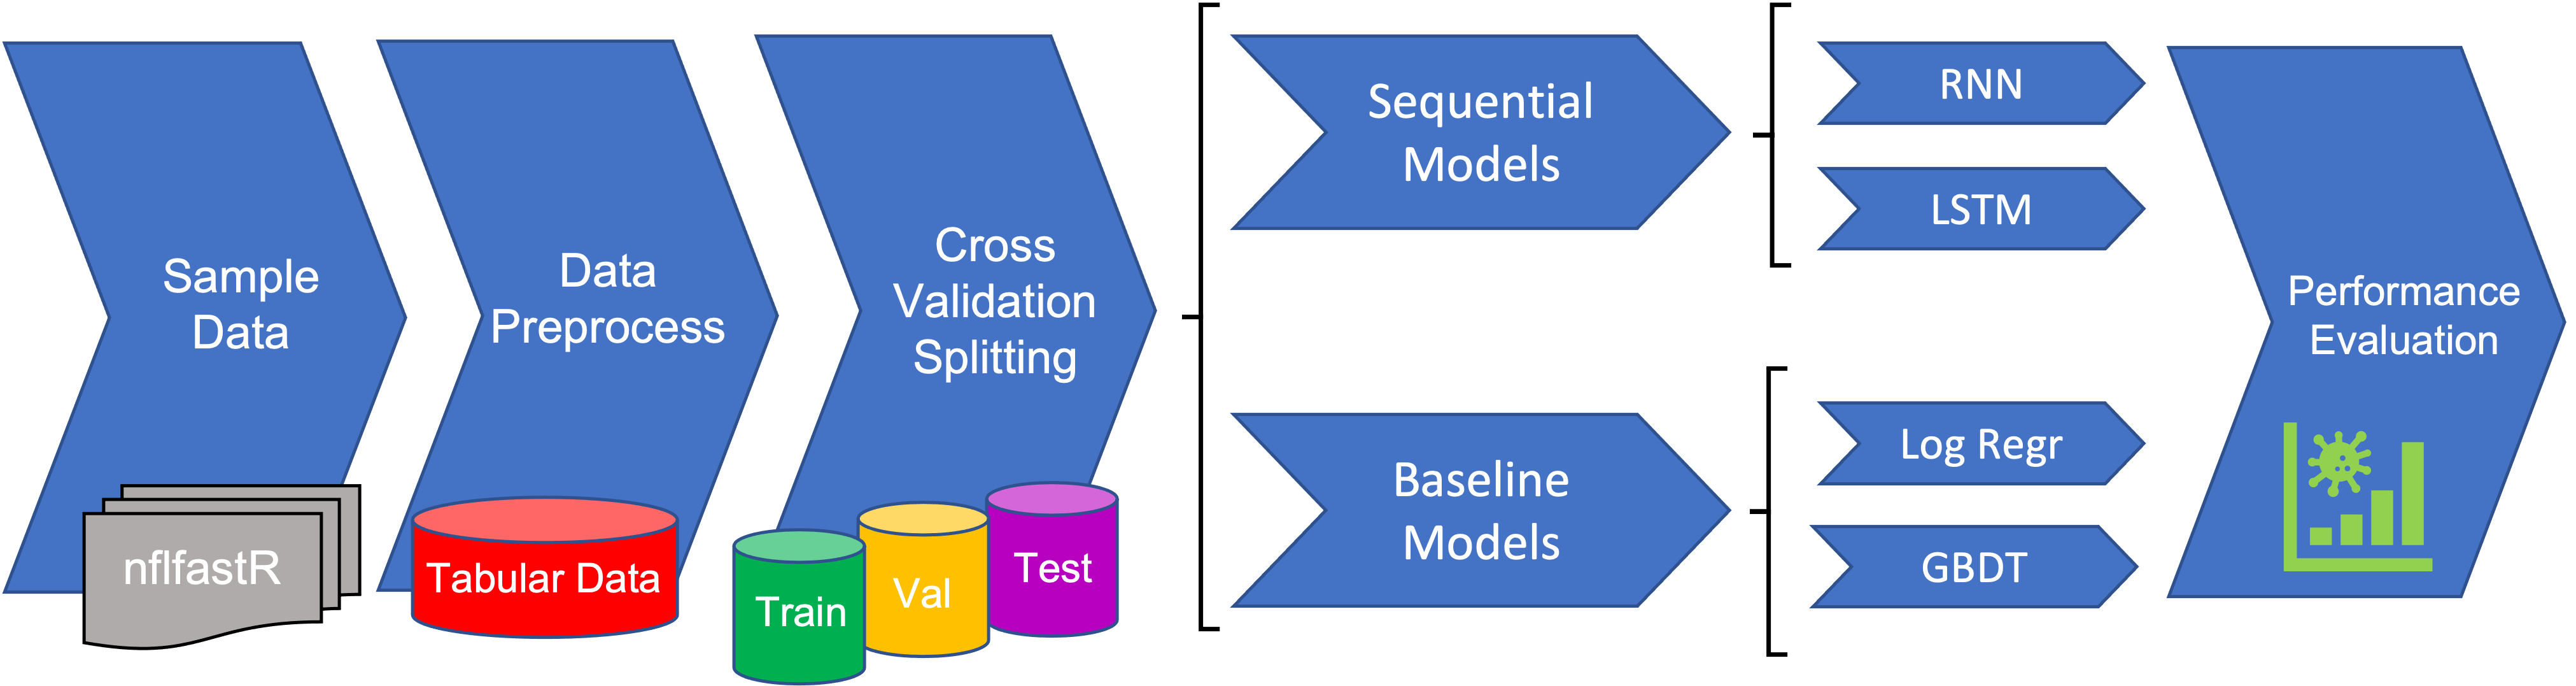
\includegraphics[width = \linewidth]{workflow.png}
            \caption{Overall Methodologic Workflow }
            \label{fig:workflow}
        \end{figure}
        \begin{multicols*}{2}

        \subsection{Preprocessing}
            \paragraph{}
                Data sampled directly from \texttt{nflfastR} contains all play types and outcomes from both the regular and post-season. 
                For the purpose of this analysis, we are only interested in regular season plays that were either passes or runs. 
                This meant removing all instances of special teams plays (kick-offs, punts, field goal attempts) and pre-snap penalties. 
                It is important to note that some plays are intended to be passes but end up being runs (this is called a QB scramble). 
                We consider these to count as passes since this was the intended play call.   
            
        \vspace{-10pt}

            \paragraph{}
                Missing values were only encountered for some of the weather features selected.
                Temperature and wind are NA for games that were played inside of a dome. 
                Inside NFL domes, the temperature is controlled and most often set to 72 degrees fahrenheit.
                Missing values for these features were set to 0 windspeed and 72 degrees fahrenheit for all play instances occurring inside a dome. 
            
        \vspace{-10pt}

            \paragraph{}
                For all methods considered, binary and categorical features need to be one-hot encoded.
                This is because machine learning models aren't able to interperet text strings directly \cite{Brownlee20}. 
                One-hot encoding entails creating a new column for each level of a categorical variable. 
                The column is a 1 if an instance falls under that category and 0 if not. 
                One-hot endcoding was chosen over integer encoding to avoid creating any ordinal pattern in the categorical features. 
        
        \subsection{Feature Engineering}
            \paragraph{} 
                Feature engineering is a vital aspect of the machine learning process. 
                It is a method by which domain knowledge is leveraged to transform raw data into meaningful features that are capable of distinguishing classes in the response.
                In this case, features are constructed to describe historical tendencies of both the offensive and defensive teams.
                This information is designed to be accurate up until the current play instance. 
            
        \vspace{-10pt} 
            
            \paragraph{}
                Cumulative tendencies are not readily available in data loaded from \texttt{nflfastR}. 
                However, enough information is included in order to build these features. 
                For the cumulative pass to run ratio, we group the data by offensive team and calculate a running total of passes ran divided by total plays. 
                This ensures the feature is current up to a given play; reflecting the information the defensive team would have before the snap. 
                Similarly, we build in features communicating the offensive teams effectiveness at either passing or running.
                The available data includes how many yards were gained for a given play. 
                Again, we group data by offensive team and calculate a runnning total of yards gained (for each type of play) divided by how many plays were ran of that type.  
                 
        \vspace{-10pt}

            \paragraph{}
                In addition to having a sense of the offensive teams tendencies and effectiveness, the defensive team will also be aware of its own weaknesses.
                This aspect is built into the data the same way as offensive tendencies. 
                Instead of grouping by offensive team, we group by defensive team and add a running total of yards allowed per play type.
        
        \subsection{Cross Validation Splitting}
            \paragraph{}
                Cross validation splitting is a method for assessing the performance of a model on unseen data. 
                The original sample of data is partitioned into three non-overlapping subsets called training, validation, and testing \cite{Haykin08}.
                Training is used for teaching the model to learn the patterns within the sample. 
                Validation is the first unseen partition and is reserved for evaluating which hyperparameter combinations perform best. 
                Hyperparameters, unlike model parameters, are not learned during the training algorithm and therefore need to be pre-specified by the user.
                Given a number of candidate models performing well on the validation set, a final performance evaluation is done on the testing data. 
                Metrics recorded at this stage are used for final reporting.

            \vspace{10pt}
                
            \begin{Figure}  
                \centering
                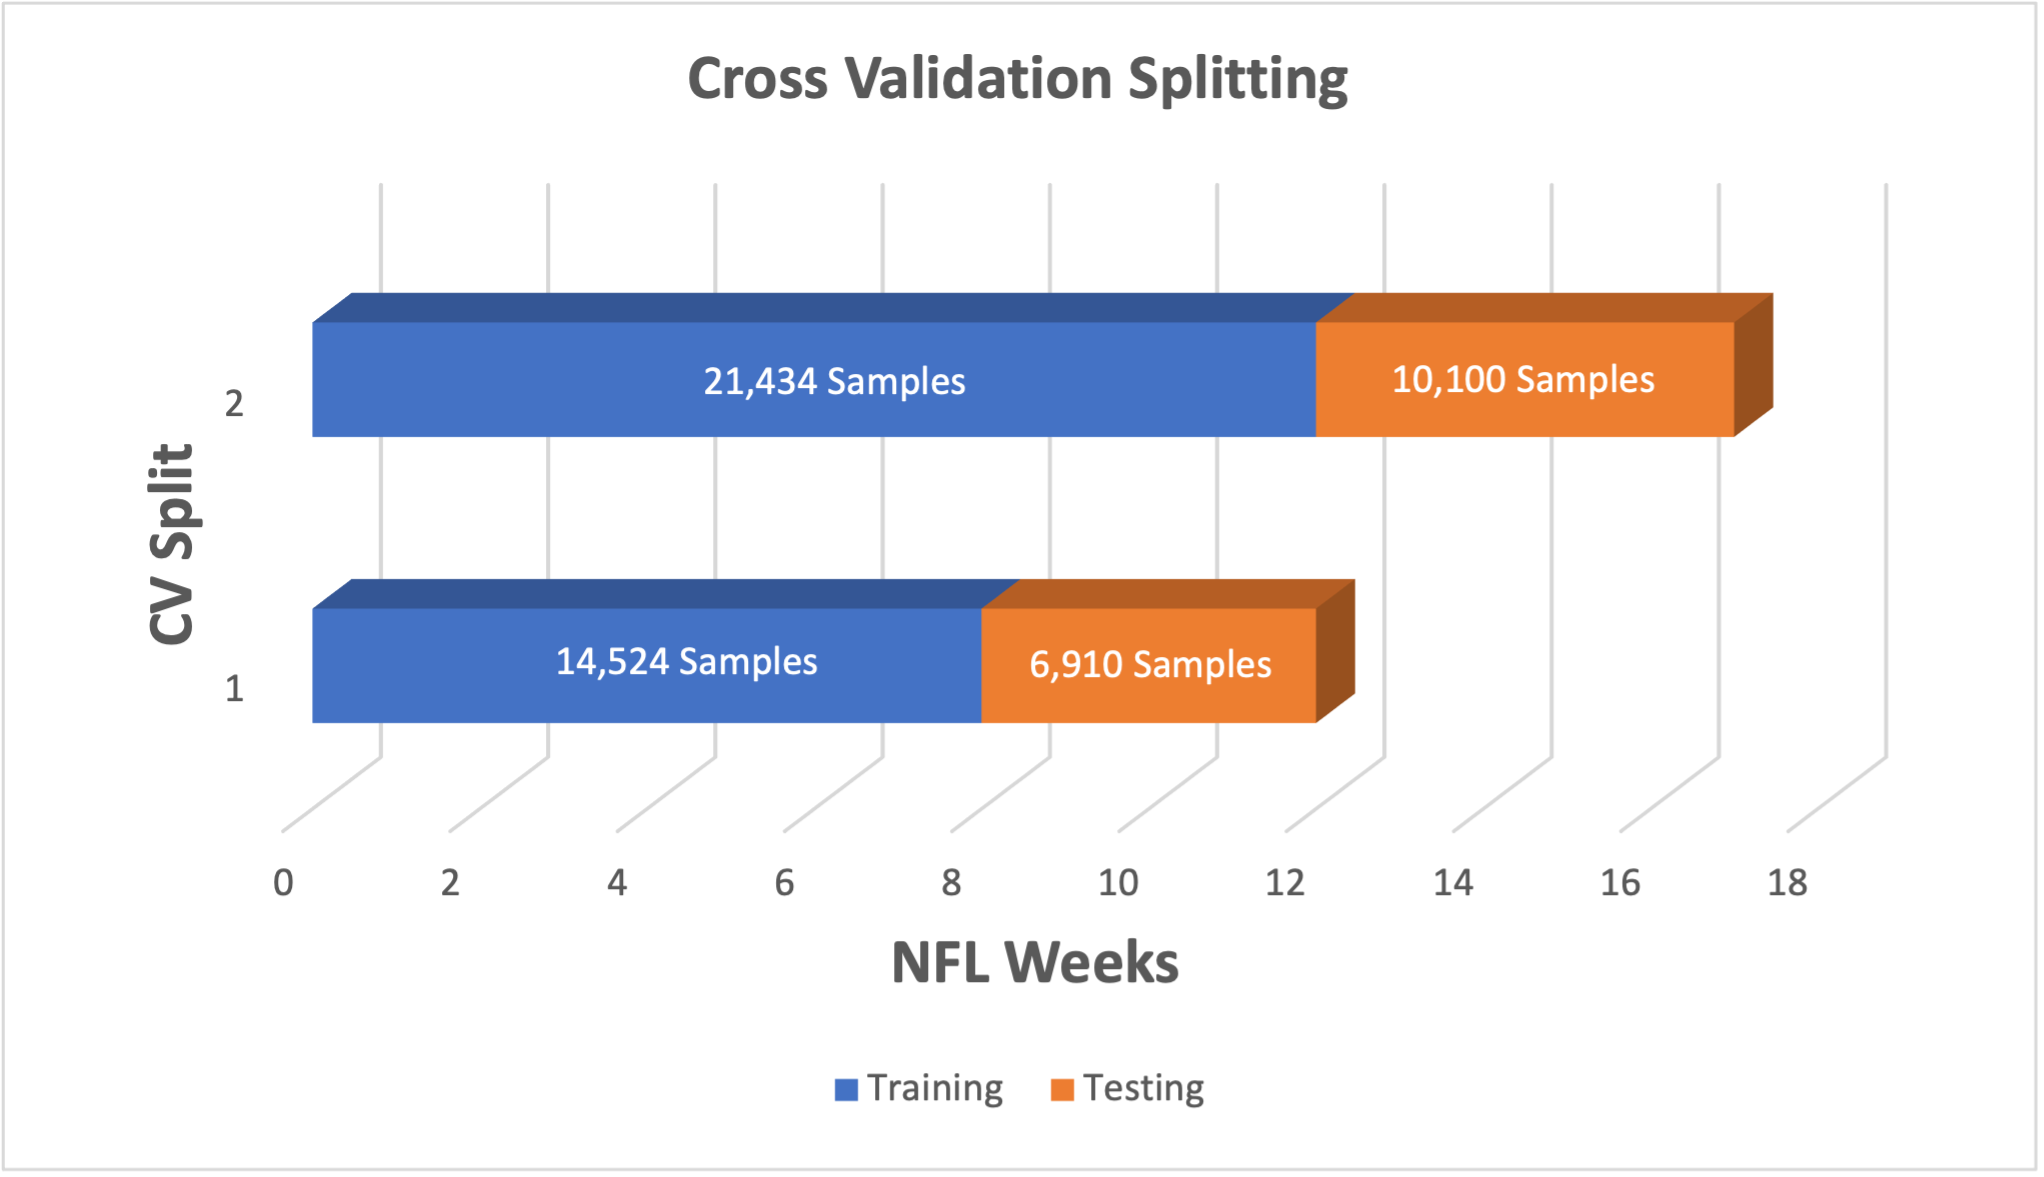
\includegraphics[width = \linewidth]{cv.png}
                \captionof{figure}{Cross Validation Splitting}
                \label{fig:Cross Validation Splitting}
            \end{Figure}

            \vspace{-10pt}

            \paragraph{}
                The cross validation scheme is described in Figure 2.
                The first 8 weeks of the NFL season are used for the training set, with weeks 9-12 as validation for evaluating hyperparameters.
                For each model type, we then select the best 20 hyperparameter combinations for testing. 
                Models with these combinations are retrained using weeks 1-12 and evaluated for final performance using weeks 13-17. 

        \subsection{Exploratory Analysis}
            \paragraph{}
                Exploring the data through table summaries and visualizations is an important step before applying any modeling strategy.
                At this stage, we analyze the distribution of the response variable as well as its relationship to the features.

            \vspace{-5pt}

            \subsubsection*{Response Variable}
                \paragraph{}
                    Understanding the distribution of the binary response variable will inform crucial aspects of applying classification models.
                    Mainly, it gives a sense of the class imbalance. 
                    Class imbalance exists in the data when one of the binary classes occurs much more often than the other. 
                    In cases with heavy imbalance (one class represents 80\% or more the observations), undersampling of the dominant class or oversampling the non-dominant class may need to be applied.
                    Table 2 shows the distribution of the response variable in the different cross validation folds.  
                
                \vspace{15pt}
                
                \begin{tabular}{|| m{2cm} | m{2cm}| m{2cm} ||}
                    \hline
                    \textbf{Fold} & \textbf{\% Pass} & \textbf{\% Run}  \\
                    \hline\hline
                    Train  & 59.50 & 40.5 \\
                    \hline
                    Validation & 60.01 & 39.99 \\
                    \hline
                    Test & 59.01 & 40.99 \\
                    \hline
                \end{tabular}
                \captionof{table}{Play Call Distribution in CV Folds}
                
                \paragraph{}
                    For the three splits, the play call distribution remains at a consistent 60-40 split in favor of passing plays. 
                    This kind of distribution is described as slightly imbalanced data. 
                    No undersampling or oversampling methods are recommended when this is the case. 
                    Note that the overall ratio of passes to runs is the same across the cross validation folds. 
                    The validation data needs to be a representative sample of the training data in order to ensure good results.
            
            \vspace{-5pt}
            \subsubsection*{Features}
                \paragraph{}
                    For brevity, only the most illuminating insights relating play calls to the features are displayed.
                    The first of which is play calls by down and distance, as illustrated in Figure 3. 
                    Notably, it is seen that runs are favored over passes on first downs, second and short, and fourth and short situations.
                    Large disparities between passes and runs exist for third/fourth and 4+ yards as well as second and long scenarios.
                    This matches what is expected as offensive teams are heavily incentivized to throw the ball on later downs and longer distances (need to gain more yards using only one or two plays). 
                    Perhaps the only surprising aspect of the plot is that passes are more common on third and short.
                    A possible explanation is that passes are being ran on third and short when the offensive team already knows it is going to go for it on fourth down (if the third down pass attempt fails). 
                    They are running the riskier option (a pass attempt) knowing they will get another try and then running the safer option (a run attempt) when there is only one attempt available.  

                \end{multicols*}
                \begin{figure}[ht]
                    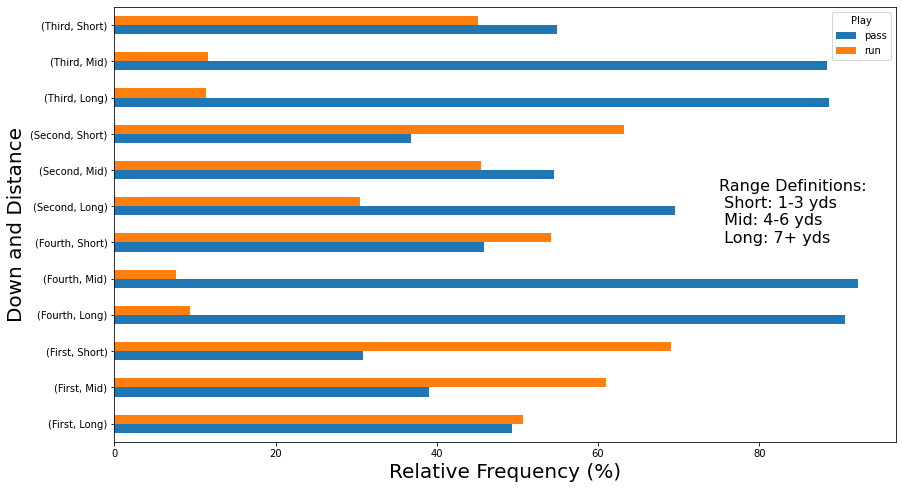
\includegraphics[width = \linewidth]{PlayCallByDownAndDist.png}
                    \caption{Relative Play Call Frequency by Down and Distance}
                    \label{fig:Play Calls}
                \end{figure}
                \begin{multicols*}{2}
                
                \paragraph{}
                    As previously mentioned, there is little information released by the NFL pertaining to what formation the offensive team lines up in.
                    However, they do release whether the play was from the shotgun formation or under center. 
                    In shotgun, the quarterback (QB) lines up farther back from the line of scrimmage. 
                    This is typically to allow more time for the QB to throw the ball before the defensive team can get to him. 
                    The relationship between shotgun formation and play type is displayed by Figure 4. 
                    For more context, the data is grouped by an additional category called huddle.
                    This binary feature tells whether the hurry-up offense is being ran. 
                    In the hurry-up, the offensive team does not meet in a huddle before running the play; this is typically done late in games to avoid losing time in between plays. 
                    The figure confirms what is expected. 
                    Passes are much more common in the shotgun formation and runs are much more common under center. 
                    They remain more common for the hurry-up offense in the shotgun formation but the same result isn't true for under center, huddle plays. 
                    It is suspected more runs are ran in this scenario because these no huddle plays are ran in normal game conditions (i.e. not with little time remaining, down by many points). 

                \begin{Figure}  
                    \centering
                    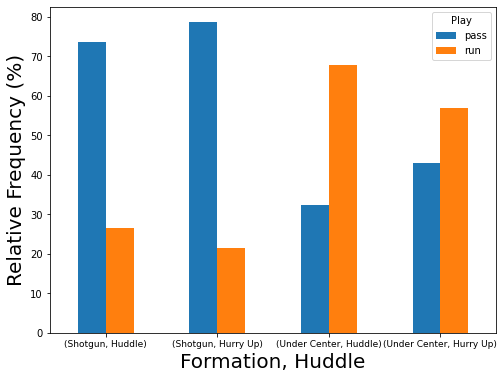
\includegraphics[width = \linewidth]{FormationHuddle.png}
                    \captionof{figure}{Play Frequency by Formation, Huddle}
                    \label{fig:Play Type by Formation and Huddle}
                \end{Figure}

                \vspace{-10pt}
                \paragraph{}
                    There is also some visible tendencies relating score differential and amount of time remaining to optimal play call decisions. 
                    This relationship is explored in Figure 5 where second half plays are examined (so that seconds remaining reflects time left in the game).
                    Passes seem to be called overwhelmingly with less than 500 seconds remaining in the game when a team is down by 0-20 points. 
                    During this same time window, runs seem to be called more when a team is leading by 0-20 points.
                    
                    \end{multicols*}
                    \begin{figure}[ht]
                        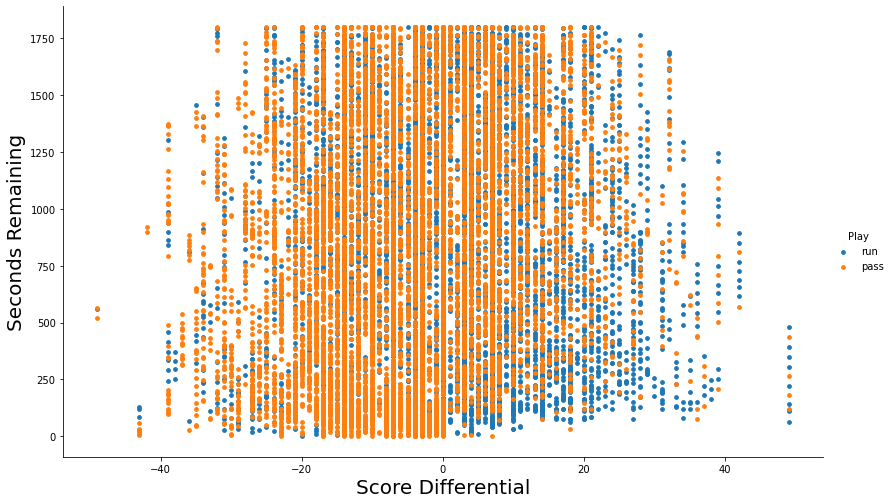
\includegraphics[width = \linewidth]{ScoreDiffSecRem.png}
                        \caption{Play Call by Score Differential and Seconds Remaining}
                        \label{fig:Play Call by Score Differential and Seconds Remaining}
                    \end{figure}
                    \begin{multicols*}{2}

                \paragraph{}
                    Finally, the evolution of play call tendencies as the season progresses are visualized in Figure 6. 
                    Teams are plotted by division (across conferences) for added visual clarity.
                    The behavior for each team is generally sporaditic for the first 1000-2000 play calls. 
                    Beyond this threshold, a given team's overall tendencies begin to steady out. 
                    In the long run it is seen that all teams operate by using around 40-80\% passing plays with most teams using about 60\%. 
                    This matches the play call distributions seen in Table 2.
                    
        
        \subsection{Sequential Models}
            \paragraph{}
                Mathematical details for the sequential neural networks used in this analysis are given. 

            \vspace{-5pt}

            \subsubsection*{Recurrent Neural Networks}
                \paragraph{}
                    Recurrent neural networks are a special class of artificial neural networks where connections between nodes flow in a consecutive sequence. 
                    This allows them to exhibit memory-like behavior and learn to understand temporal patterns. 
                    While originally intended for speech and text recognition \cite{Li15}, they have been applied to a multitude of tasks where data represents a time series.
                
                \vspace{-10pt}

                \paragraph{}
                    For the models used in this work, let the pair $(X_i, y_i)$ for $i = 1,2,...N$ represent a training observation where:
                    
                    \begin{itemize}
                        \item $X_i := X_{t-k}^m, X_{t-k+1}^m, ... , X_{t}^m$ i.e. a sequence (size $k$) of design vectors (dimension $m$, the number of features)  
                        \item $y_i := y_{t}$ i.e. the binary response at time $t$ 
                    \end{itemize}

                    Importantly, each input represents a sequence of feature vectors of length $k$ while the target is the binary label at the end of each sequence. 
                    Hence, in the context of this analysis, the previous $k$ play calls and current conditions are used to predict the play at timestep $t$. 
                    Now define a simple recurrent network connecting the sequence of inputs to the outputs \cite{Dupond19}:

                    \begin{itemize}
                        \item $h_t = \sigma_{h}(W_{h}X_{t} + U_{h}h_{t-1} + b_{h})$ 
                        \item $\hat{y_t} = \sigma_{y}(W_{y}h_{t} + b_{y})$ 
                    \end{itemize}

                    Where the variables are given by:



            \end{multicols*}
            \begin{figure}[ht]
                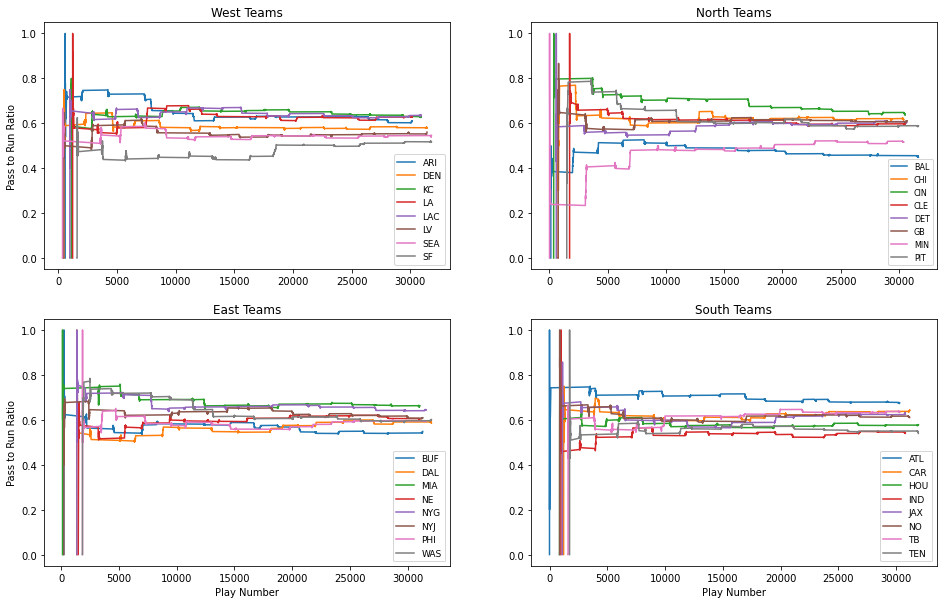
\includegraphics[width = \linewidth]{ptr.png}
                \caption{Pass to Run Ratio by Team}
                \label{fig:Pass to Run Ratio by Team}
            \end{figure}
            \begin{multicols*}{2}

                    \begin{itemize}
                        \item $X_t: $ Input matrix 
                        \item $h_t := $ Vector of hidden states
                        \item $W_h := $ Weights connecting inputs to hidden states
                        \item $U_h := $ Weights connecting hidden states to previous hidden states
                        \item $b_h := $ Hidden state biases
                        \item $W_y := $ Weights connecting hidden states to outputs
                        \item $b_y := $ Output biases
                        \item $\sigma_h := $ Hidden state activation function
                        \item $\sigma_y := $ Output activation function
                        \item $\hat{y_t} := $ Predicted target variable
                    \end{itemize}

                \paragraph{}
                    A visual representation of the network is given in Figure 7. 
                    Note this is a many to one network. 

                \begin{Figure}  
                    \centering
                    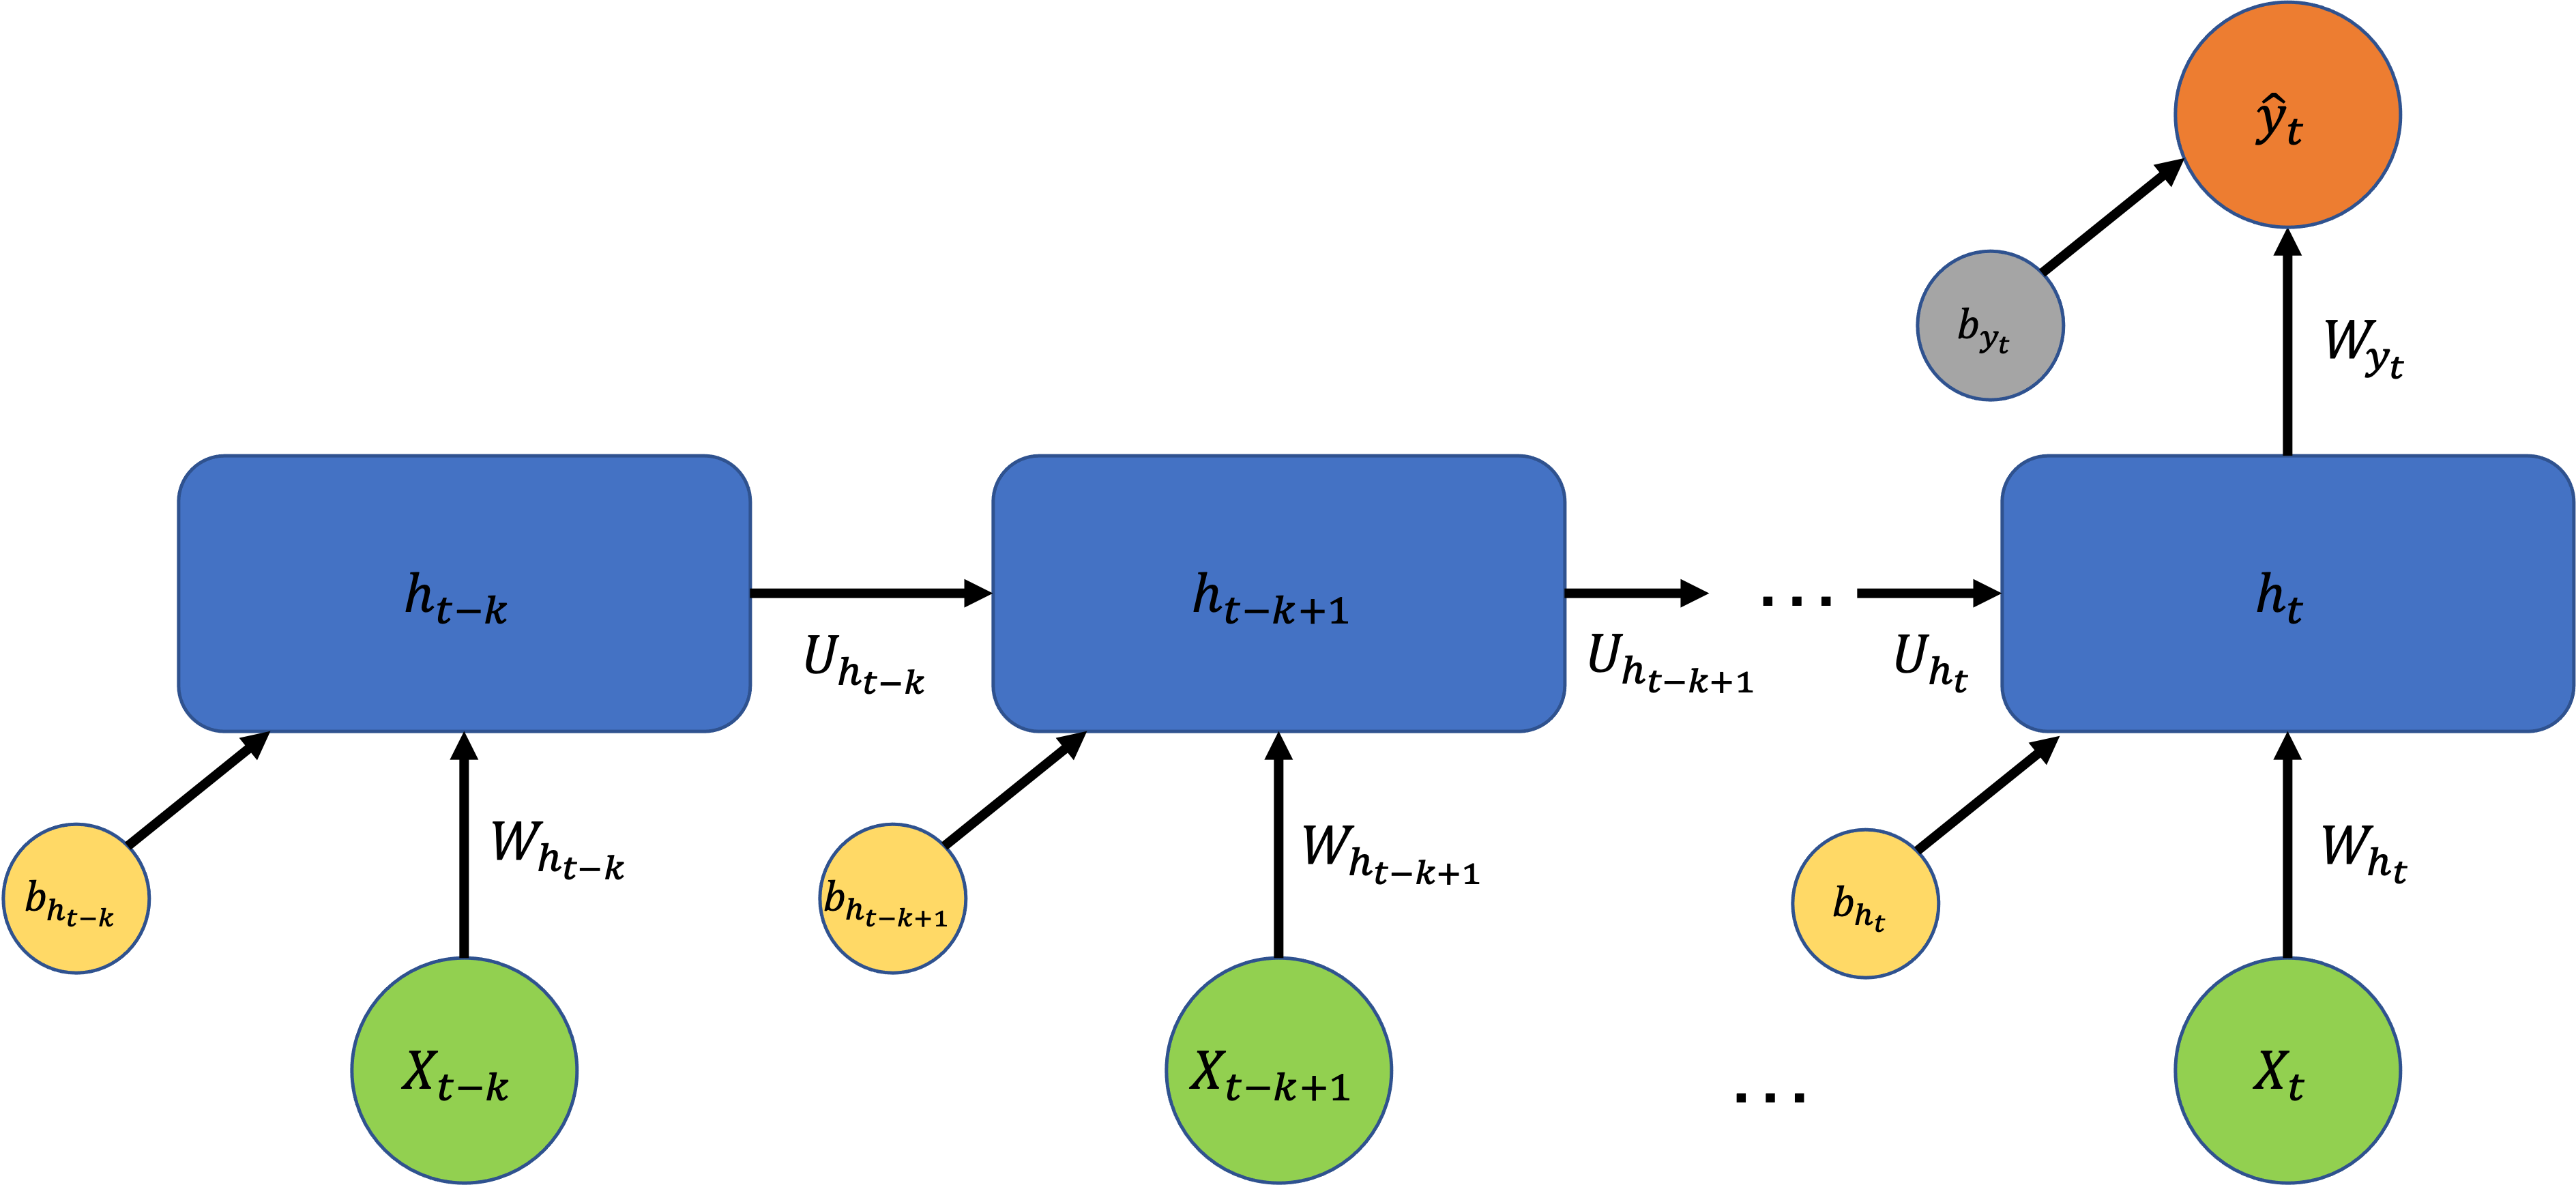
\includegraphics[width = \linewidth]{rnnStructure.png}
                    \captionof{figure}{Basic RNN Topology}
                    \label{fig:Basic RNN Topolgy}
                \end{Figure}

                \vspace{-5pt}

                \paragraph{}
                    Activation functions are used to map resulting values (hidden or output states) to a normalized range (usually (0,1) or (-1,1)) \cite{Murilo22}.
                    For hidden state activation, the choice of hyperbolic tangent (tanh) and exponential linear unit (elu) functions are tuned as hyperparameters, while sigmoid is used for the outputs:
                    
                    \begin{itemize}
                        \item tanh $:= \sigma(z) = \frac{e^z - e^{-z}}{e^z + e^{-z}}$ 
                        \item elu $:= \sigma(z) = \alpha(e^z - 1) \hspace{0.2cm} if \hspace{0.2cm} z \le 0, \hspace{0.2cm} z \hspace{0.2cm} else$
                        \item sigmoid $:= \sigma(z) = \frac{1}{1 + e^{-z}}$
                    \end{itemize} 

                    While the simple RNN structure suffices for showing the mathematical details, it should be noted that added complexity is used for modeling in this work.
                    This includes stacking multiple recurrent and dense layers before the output layer. 
                    When this is the case, the outputs of the previous layer simply feed into the next one.
                    Many such aspects of the model topology are treated as hyperparameters, as will be discussed later on.
                
                \vspace{-10pt}

                \paragraph{}    
                    For training a recurrent network, a first order iterative optimization algorithm known as mini-batch gradient descent is used with backpropogation \cite{Mozer95}. 
                    First, define a cost function $C(y_i, \hat{y_i})$ relating model predictions to actual observed outcomes. 
                    The cost function is designed to be large when the model missclassifies an observation and small when it correctly classifies. 
                    In this analysis the binary cross entropy (also known as log-loss) cost function is used: $$C(y_i, \hat{y_i}) = -(y_i log(\hat{y_i}) + (1 - y_i)log(1 - \hat{y_i}))$$
                    The value for $\hat{y_i}$ is between 0 and 1, interpreted as the predicted probability the observation belongs to a given class.
                    As $C(y_i, \hat{y_i})$ is a function of model parameters (weights and biases), optimal parameters are found by minimizing the cost function.
                    
                \vspace{-10pt}

                \paragraph{}
                    Given a choice of cost function, the training algorithm begins by randomly sampling observations from the sample into mini-batches of size $n$.
                    This is done for managing computational efficiency while ensuring convergence to a global minimum.  
                    It is common practice to set $n = 32$ as is done in this work.
                    For each mini-batch the weights and biases must first be set to initial values, this is done by randomly sampling from a uniform distribution.
                    A forward pass is completed given these initial values, hence all hidden state and output activations are computed.
                    Given model outputs, the gradient of the cost function with respect to model parameters across all samples in the mini-batch is attained. 
                    A backward pass is then performed by updating the weights and biases according to the negative direction of the gradient and a pre-specified learning rate $\gamma$. 
                    Parameters are updated as follows: $$\bar{\Theta}_{j+1} = \bar{\Theta}_j - \gamma (\nabla C(\bar{\Theta}_j))$$

                \paragraph{}
                    When the model completes a mini-batch, it is called an iteration. 
                    The algorithm will then continue through all mini-batches to complete an epoch (i.e. it has seen all observations in the training sample).
                    This process will repeat for a pre-specified number of epochs or until a stopping cirteria is met.
                    Typically, this criteria is to stop when the cost function has not reduced over a given number of epochs. 
                    

            \vspace{-5pt}

            \subsubsection*{LSTM Neural Networks}
                \paragraph{}
                    A problem with traditional RNNs is that they struggle to pick up on long term patterns.
                    LSTM models have a similar structure with some added complexity that tries to account for long dependencies. 
                    Let the training observation pairs be represented by $(X_i,y_i)$ as they were previously.
                    Define a new network relating the input sequence to the output \cite{Dupond19}:

                    \begin{itemize}
                        \item $f_t = \sigma_{g}(W_{f}X_{t} + U_{f}h_{t-1} + b_{f})$ 
                        \item $p_t = \sigma_{g}(W_{p}X_{t} + U_{t}h_{t-1} + b_{p})$
                        \item $\tilde{c_t} = \sigma_{c}(W_{c}X_{i} + U_{c}h_{t-1} + b_{c})$ 
                        \item $c_t = f_t \circ c_{t-1} + p_t \circ \tilde{c_t}$
                        \item $h_t = o_t \circ \sigma_c(c_t)$
                        \item $o_t = \sigma_{g}(W_{y}X_{t} + U_{y}h_{t-1} + b_{o})$
                    \end{itemize}

                    Where the variables are defined as follows:

                    \begin{itemize}
                        \item $f_t := $ Forget gate   
                        \item $p_t := $ Update gate
                        \item $\tilde{c_t} := $ Cell update  
                        \item $c_t := $ Cell state
                        \item $h_t := $ Hidden state
                        \item $o_t := $ Output gate
                        \item $W,U,b := $ Weights and Biases
                        \item $\sigma_g := $ Sigmoid activation
                        \item $\sigma_c := $ Hyperbolic Tangent activation
                        \item $\circ := $ Pointwise vector multiplication
                    \end{itemize}

                    \end{multicols*}
                    \begin{figure}[ht]
                        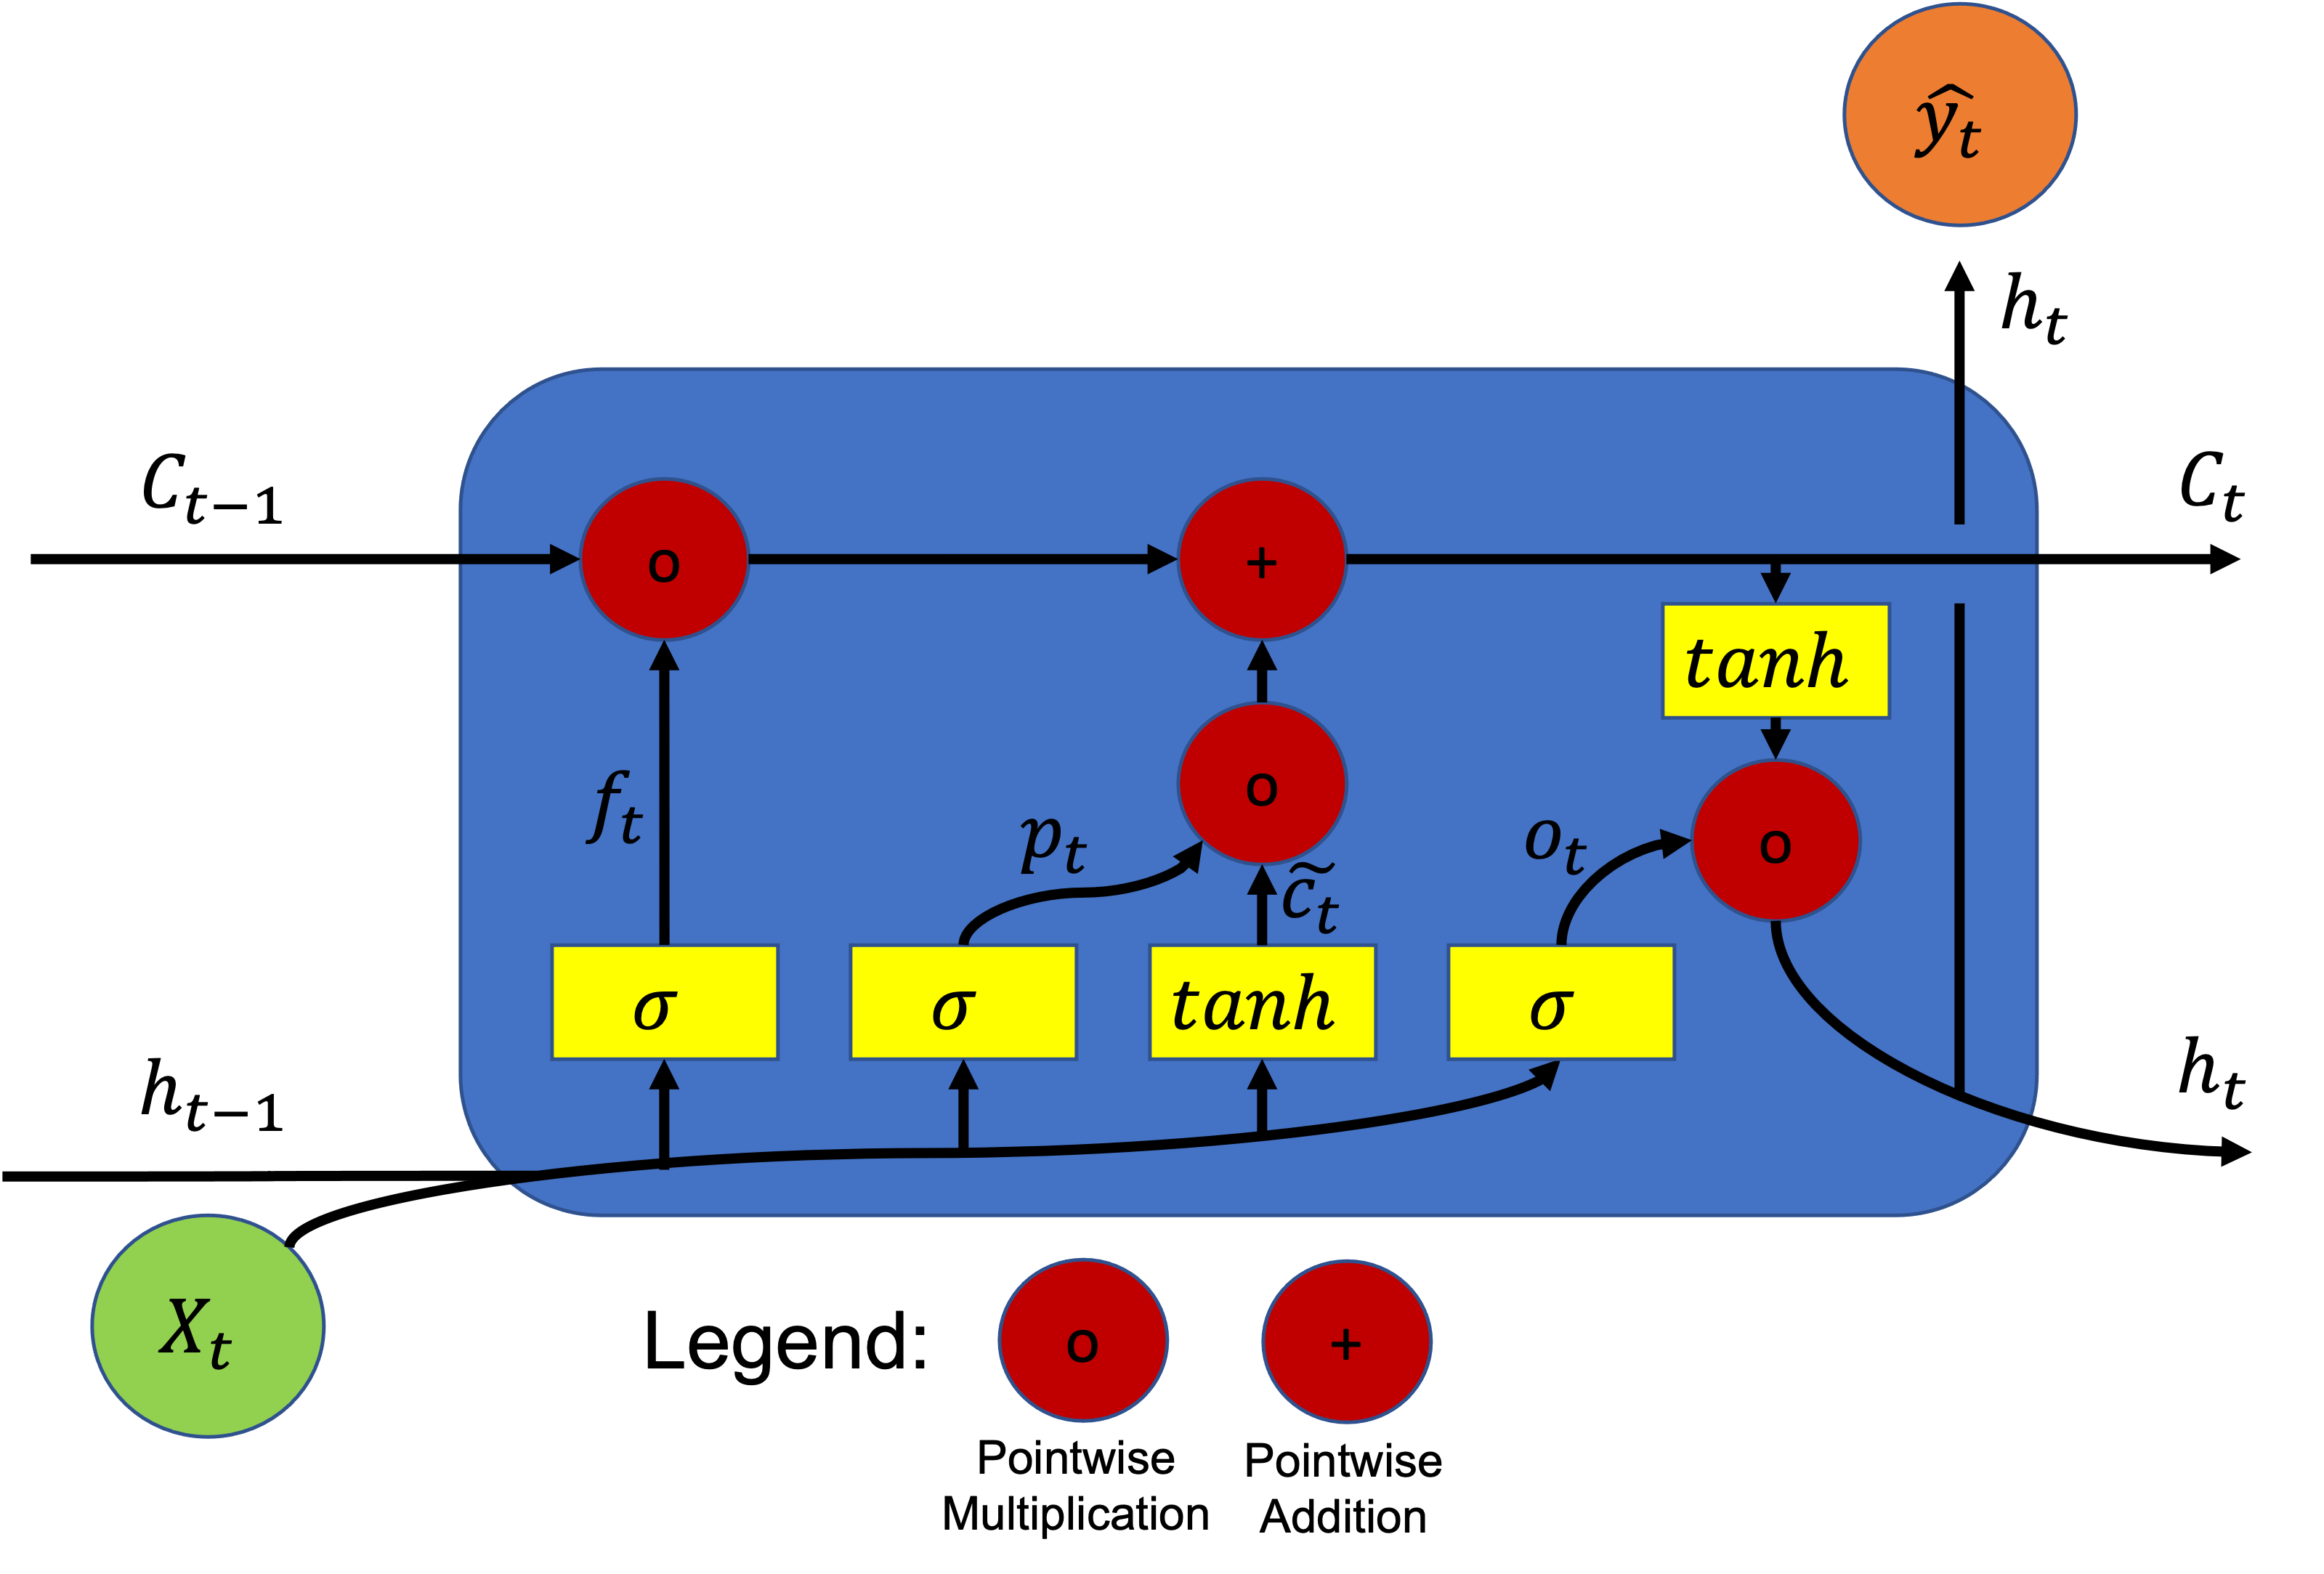
\includegraphics[width = \linewidth]{lstmStructure.png}
                        \caption{LSTM Topology}
                        \label{fig:LSTM Topology}
                    \end{figure}
                    \begin{multicols*}{2}

                    \paragraph{}
                        The structure of an LSTM cell is shown in Figure 8.
                        The cell state $c_t$ communicates the long term memory of the network and is updated at various points within the cell.  
                        $f_t$, the forget gate, is used for deciding what to discard.
                        It combines information from the previous output and the current input and uses sigmoid activation to compress this into a value between 0 and 1.
                        This is combined with $c_{t-1}$, the previous cell state, by pointwise multiplication.
                        Values close to 1 mean keep this information while values close to 0 mean discard it. 
                        
                    \vspace{-10pt}

                    \paragraph{}
                        Then, new information is added to the cell state by pointwise multiplication of an input gate layer $p_t$ (sigmoid activation) and candidate cell values $\tilde{c_t}$ (tanh activation).
                        The cell update values combine information from the previous cell and current input while the input gate scales how much influence the update should have on the cell state.
                        After this is decided, this information is added to the cell state by pointwise addition.

                    \vspace{-10pt}

                    \paragraph{}
                        Given that the cell state has been updated, the cell must now decide what information to output.
                        The output gate, $o_t$, uses sigmoid activation to transmit information from the previous outputs and current input.
                        This is merged with information from the updated cell state (tanh activation) by pointwise multiplication.
                        Output is passed to the next LSTM cell (along with the updated cell state) and to the current target prediction \cite{Olah15}.
                        
                    \vspace{-5pt}

                    \paragraph{} 
                        The training process for LSTM neural networks is the same as in simple RNNs. 
                        Mini-batch gradient descent with backpropogation is used with the same cost function (binary cross entropy) to train all weights and biases.
                        As is the case with RNNs, added complexity of LSTM topology is explored in this analysis.
                        The structure of a sequential model, whether LSTM or RNN, is tuned via various a hyperparameters.
                        A list of hyperparameters chosen for model tuning of sequential neural networks is given in Table 3. 

                    \end{multicols*}
                    \begin{table*}[ht]
                    \caption{Sequential Model Hyperparameters} \label{tab:Sequential Model Hyperparameters} 
                    \centering
                    \begin{tabular}{|| m{3cm} | m{8.75cm}| m{2cm} | m{1.25cm} |}
                        \hline
                        \textbf{Parameter} & \textbf{Description} & \textbf{Range} & \textbf{Model} \\
                        \hline\hline
                        Sequence Length & (int) k, Number of plays to consider a sequence & [1,15] & Both \\
                        \hline
                        Sequential Layers & (int) Number of LSTM or RNN layers to stack & [1,4] & Both \\
                        \hline
                        Recurrent Units & (int) Number of hidden states in sequential models & [8,102] & Both \\
                        \hline
                        RNN activation & (choice) Hidden state activation for RNNs & [tanh, elu] & RNN \\
                        \hline
                        RNN dropout & (float) Fraction of units to drop from input & [0.1,0.25] & RNN \\
                        \hline
                        RNN rec dropout & (float) Fraction of units to drop from recurrent states & [0.1,0.35] & RNN \\
                        \hline
                        LSTM dropout & (float) Fraction of units to drop from input & [0.1,0.25] & LSTM \\
                        \hline
                        Dense layers & (int) Number of dense layers after sequential layers & [1,2] & Both \\
                        \hline
                        Dense dropout & (float) Fraction of input units to drop (dense layers) & [0.1,0.3] & Both \\
                        \hline
                        Learning rate & (float) Rate at which weights are updated in training & [$1e^{-5},1e^{-2}$] & Both \\
                        \hline
                    \end{tabular}
                    \end{table*}
                    \begin{multicols*}{2}

                    \paragraph{}
                        The use of dropout at various stages warrants further explanation. 
                        This is a regularization parameter. 
                        Regularization refers to measures in machine learning algorithms that counteract overfitting \cite{Hastie01}.
                        Overfitting occurs when a model fits too closely to the training data and therefore doesn't generalize well to new observations.
                        When dropout is added to a layer in a deep learning model, the fraction sets the amount of randomly selected inputs to turn off (set to 0). 
                        This helps to avoid keying in to closely to the training inputs and helps performance on test data. 

        \subsection{Baseline Models}

            \subsubsection*{Logistic Regression}
                \paragraph{}
                    Logistic regression is a simple but powerful classification algorithm that is applied in a wide range of contexts \cite{Hastie01}.
                    In this setting, each data point $(X_i,y_i)$, $i = 1,...,N$ is treated as an individual play call and feature vector (i.e. not a sequence).
                    Arrange the feature vectors into an $N \times m$ design matrix $X$ and define a column parameter vector $\beta$ of length $m$.
                    The parameters describe the relationship between each feature and the response.
                    The probability that the response belongs to the positive class at each $i$ is then given by:
                    
                    $$\hat{y} = \sigma_g(X\beta)$$

                    Where $\sigma_g$ is the sigmoid activation function defined earlier. 
                    Similarly to the training of sequential models, a cost function is defined $C(y_i, \hat{y_i})$.
                    Again, the binary cross entropy is chosen as the cost function. 
                    Gradient descent is applied in this context as well as once more the task is to find optimal parameters that minimize the cost function.
                    The parameters are initialized at random.
                    Then, at each training iteration, the parameters are updated by the gradient of the cost function given a specified learning rate $\gamma$:

                    $$\beta_{j+1} = \beta_j - (\gamma \nabla C(\beta_j))$$

                    This process is repeated for a specified number of iterations or until a similar stopping condition as in sequential models. 

            \subsubsection*{Gradient Boosted Decision Trees}
                \paragraph{}
                    Gradient boosted decision trees (GBDT) are a popular class of ensemble models \cite{Hastie01}. 
                    They are called an ensemble because they combine the predictions of many so called weak learners. 
                    Weak learners in this context are decision tree classifiers. 
                    Decision trees work by partitioning the feature space into subregions that seek to seperate the target classes.
                    This is done by a series of binary decisions pertaining to certain values of the features. 
                    For an in context example, the model might first consider splitting observations based on time remaining in the game. 
                    All obervations falling under 250 seconds are sent down one branch of the tree and the rest another. 
                    For observations under 250 seconds, another split might be considered based on score differential, whether it is positive or negative.
                    This example is illustrated by the tree diagram in Figure 9.
                    
                    \begin{Figure}  
                        \centering
                        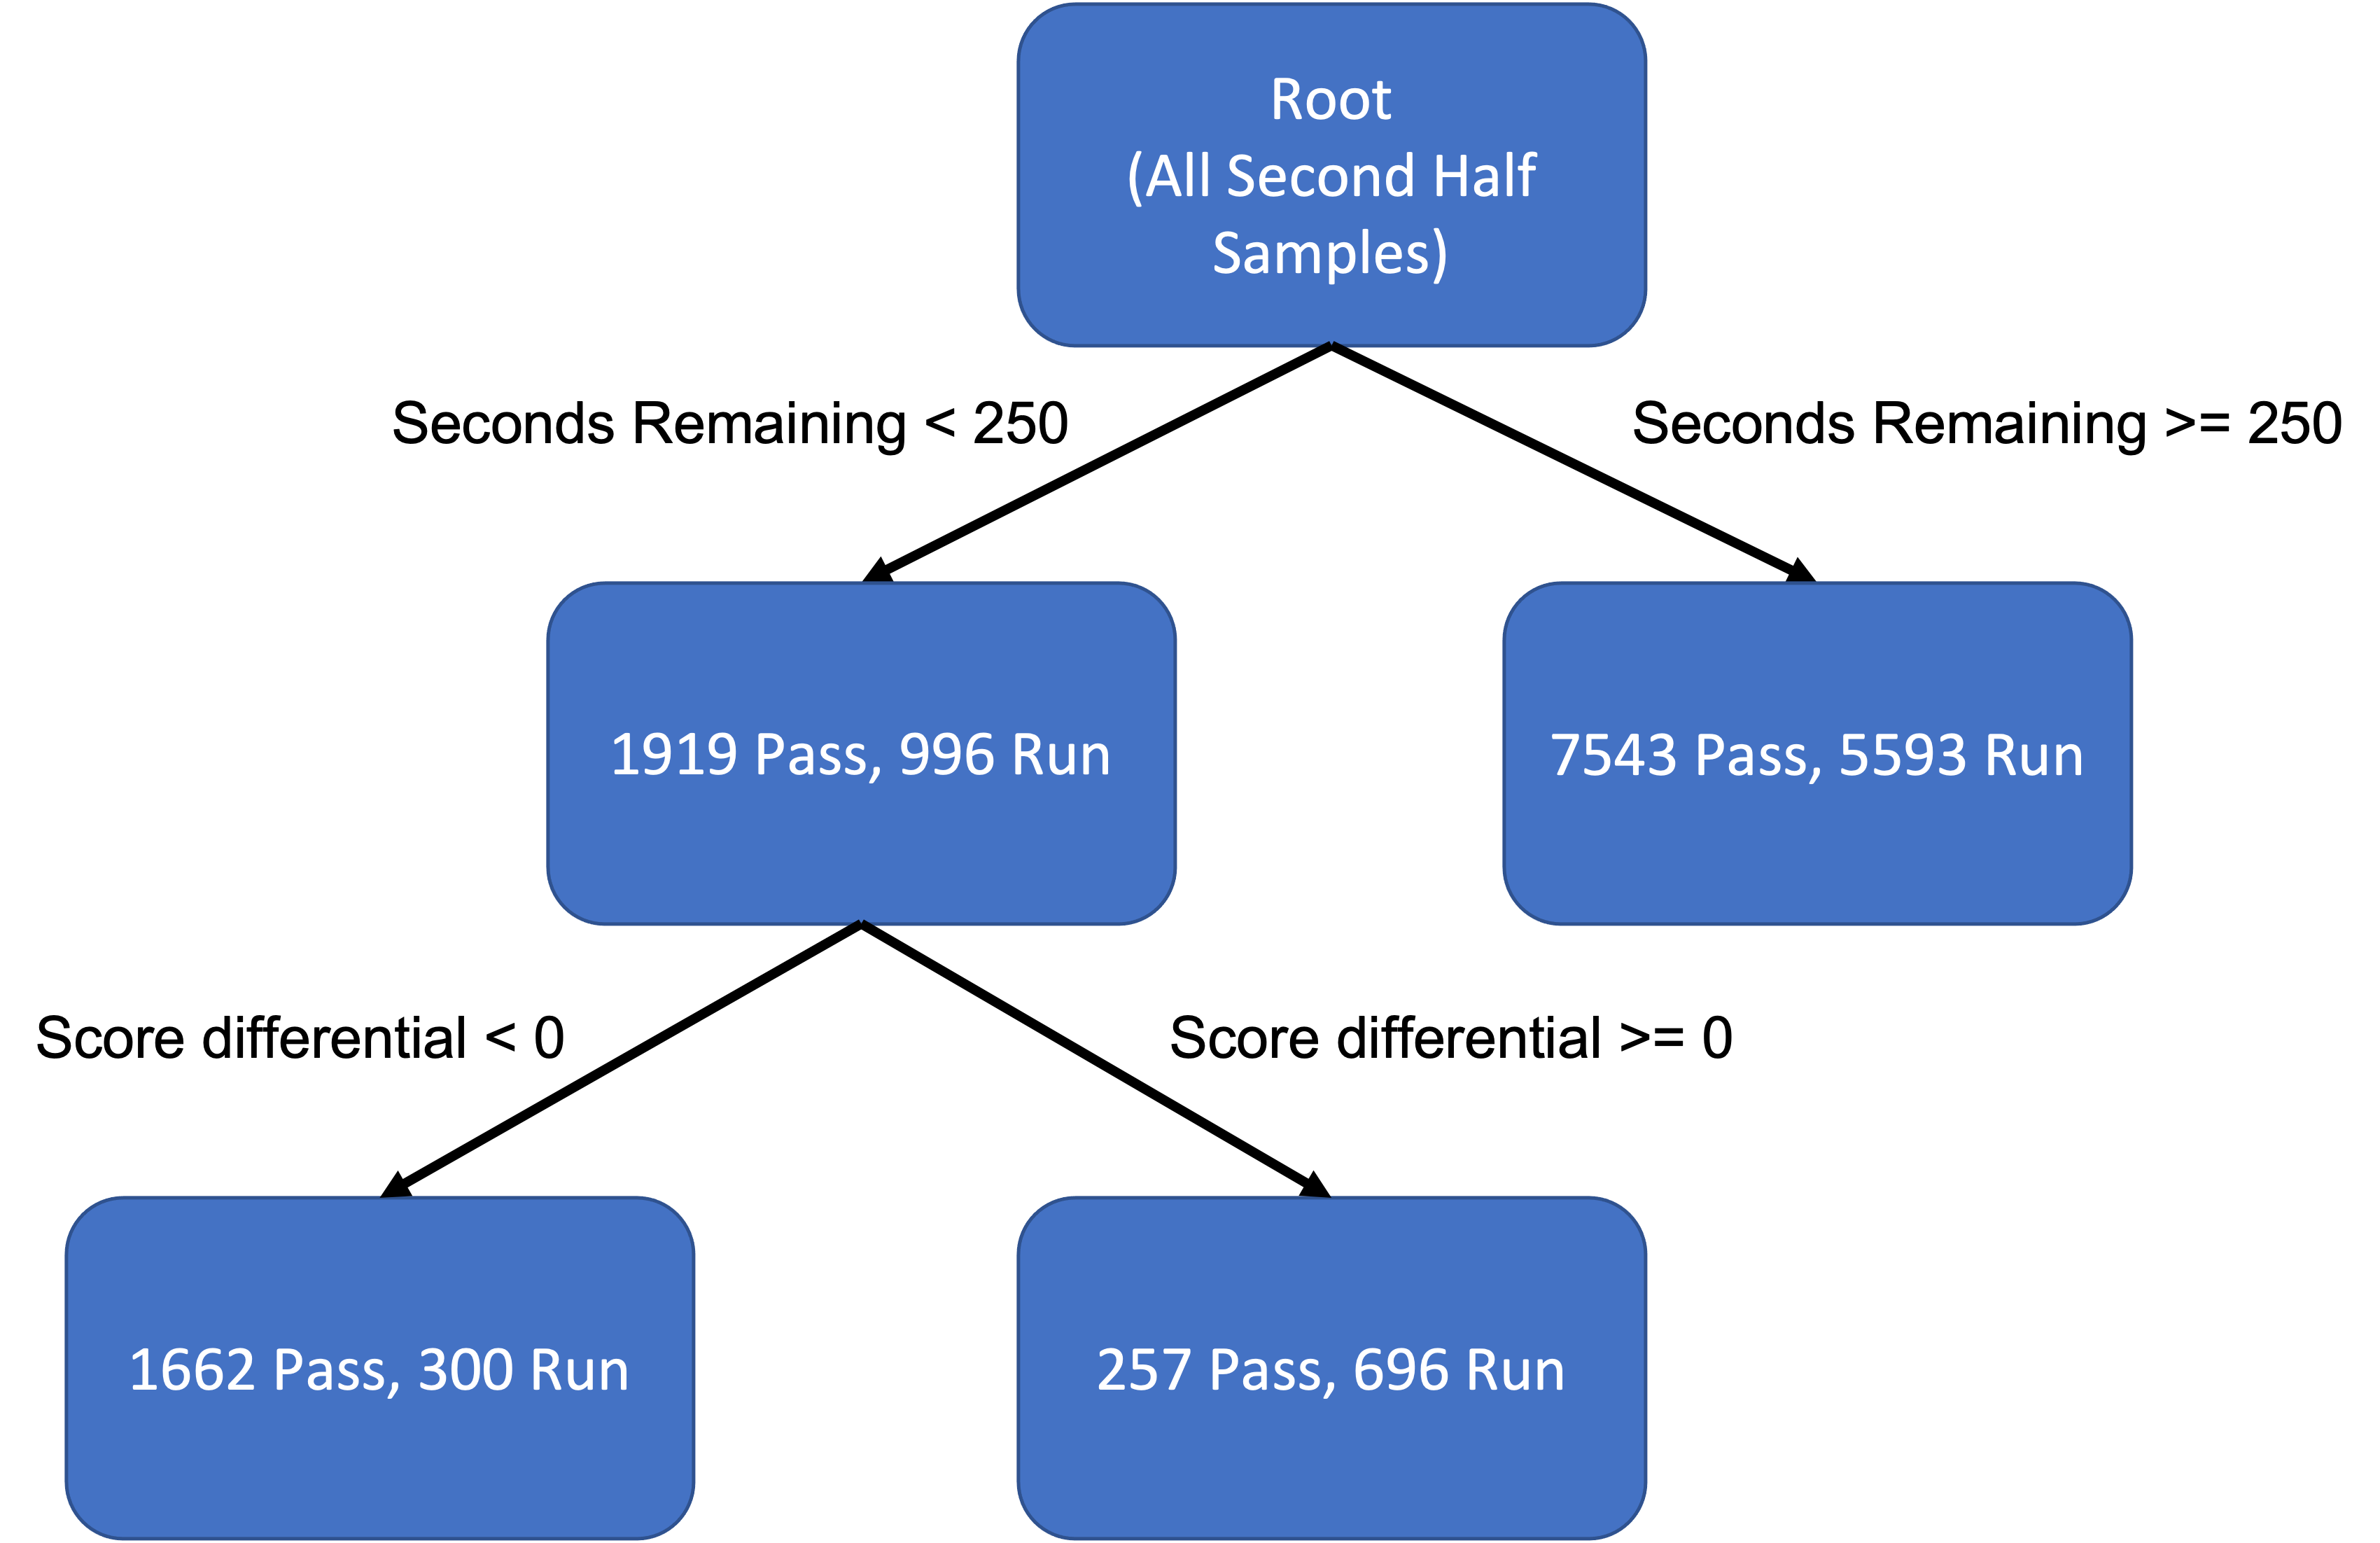
\includegraphics[width = \linewidth]{treeDiagram.png}
                        \captionof{figure}{Simple Tree Diagram}
                        \label{fig:Simple Tree}
                    \end{Figure}

                    
                \paragraph{}
                    The quality of a subregion is assessed by the binary cross entropy (as defined earlier) of observations that fall within its range. 
                    Determining optimal parameters (where to make splits, what features to use for a split, and what threshold of said features) is done by a greedy optimization algorithm.
                    It starts from a single root branch and adds branches in an iterative fashion, making locally optimal decisions at each step. 
                    Predictions are made by majority voting in the leaf nodes and the probability of belonging to a class is given by its proportion of observations in the leaf. 
                    
                \vspace{-10pt}

                \paragraph{}
                    Decision trees are considered weak learners because they exhibit a lot of variance based on the training data used. 
                    This means that using a different sample of training data will dramatically change the structure of the tree, causing the tendency to overfit.
                    To overcome this defect, single decision tree models are rarely used, and instead multiple are combined in various ways called ensembles. 
                    Gradient boosting is one such ensemble method that builds multiple decision trees in an iterative fashion, with each iteration correcting the mistakes of it predecessor.

                \vspace{-10pt}

                \paragraph{}
                    As the name suggests, another form of the gradient descent algorithm is used for optimization.
                    Letting the data be represented by $(X_i,y_i)$, $i=1,..,N$, let $\gamma$ denoted the log(odds) of the target variable i.e. $log(\frac{passes}{runs})$.
                    Define a cost function as: $$C(y_i, \gamma) = -y_i\gamma + log(1+e^\gamma)$$
                    The process begins by determining an initial model defined by a single constant leaf node for all $N$ observations. 
                    This is done by minimizing $\gamma$ over the sum of the cost function across $N$: $$M_0 = argmin_\gamma \sum_{i=1}^N C(y_i, \gamma)$$ 
                    Where $M_0$ represents the initial model. 
                    Given this choice of loss function, the value for $\gamma$ that minimizes this sum is simply the log(odds) based on observed values in the data.
                    The model iterates by fitting decision trees to residuals between observed values and the previous probability predictions.
                    For $j=1,...,J$:

                    \begin{enumerate}
                        \item Find the residual $r_{ij} = -\frac{\partial C(y_i,M_{j-1}(X_i))}{\partial M_{j-1}}$
                        \item Fit a decision tree using the features and the residuals $(X_i,r_{ij})$
                        \item Calculate output values in the new decision tree $\gamma_j = argmin_\gamma \sum_{i=1}^N C(y_i, M_{j-1}(X_i) + \gamma h_j(X_i))$ 
                        \item Update the model $M_j = M_{j-1} + \gamma_j h_j$
                    \end{enumerate}

                    The final model ouput will be $M_J$.
                    Step 4 can be seen to closely resemble the prior results of gradient descent where $\gamma_j$ represents the learning rate.
                    
                \vspace{-10pt}

                \paragraph{}
                    As was the case with sequential models, there are a number of hyperparameters to tune in both logistic regression and gradient boosted decision trees.
                    A list of hyperparameters for the baseline models is given in Table 4. 
                    Again, many of these are related to regularization. 
                    In logistic regression, this comes in the form of an elastic net. 
                    An elastic net is a way to penalize the cost function by mixing $L_1$ and $L_2$ norms. 
                    The ratio controls how much $L_1$ penalization to use relative to $L_2$. 
                    Penalization constrains the parameters during optimization and forces the algorithm to favor more simplistic models, which helps if the model overfits. 
                
                \vspace{-10pt}
                
                \paragraph{}
                    For GBDT, there are a number of regularization parameters. 
                    A random subsample (with replacement) of the original data is used during the bulding of each tree.
                    This is akin to bootstrapping and greatly decreases the variance of predictions given a change in training data. 
                    Similarly, only a random subsample of features are considered at each split (the square root of the total features).   
                    Aspects of the tree structure such as the minimum
                        
            \end{multicols*}
            \begin{table*}[ht]
            \caption{Baseline Model Hyperparameters} \label{tab:Baseline Model Hyperparameters} 
            \centering
            \begin{tabular}{|| m{3cm} | m{8.75cm}| m{2cm} | m{1.25cm} |}
                \hline
                \textbf{Parameter} & \textbf{Description} & \textbf{Range} & \textbf{Model} \\
                \hline\hline
                Estimators & (int) Number of iterations  & [100,500] & GBDT \\
                \hline
                Subsample & (float) Fraction of samples to consider for each tree & [0.5,1.0] & GBDT \\
                \hline
                Min samples split & (int) Min number of samples needed to split a node & [2,15] & GBDT \\
                \hline
                Min samples leaf & (int) Min number of samples needed in each leaf & [1, 10] & GBDT \\
                \hline
                Max Depth & (int) Max number of consecutive branches & [1,5] & GBDT \\
                \hline
                $L_1$ ratio & (float) Proportion of $L_1$ penalty to $L_2$ & [0,1] & LOG \\
                \hline
            \end{tabular}
            \end{table*}
            \begin{multicols*}{2}

            
            \noindent samples needed to make a split, minimum samples required in a leaf, and max depth all prevent the model from learning the training data too closely.
            
            
        \subsection{Tuning Algorithm}
            \paragraph{}
                Model tuning is a procedure where different hyperparameter combinations are tested on validation data. 
                There are a number of ways to conduct this process.
                Given extensive search spaces (possible parameter combinations) and limited computational resources, a tuning algorithm with optimal efficiency is favored.
                This analysis used a Hyperband search strategy. 
                
            \vspace{-10pt}

            \paragraph{}
                Hyperband is designed to allocate more resources (i.e. training iterations) to models that are promising in their early stages. 
                The algorithm builds off the idea of successive halving \cite{Jameison17}.
                In successive halving, a large number of randomly chosen combinations are ran for a few iterations. 
                The top half performing combinations are chosen to continue training for more iterations and the rest are discared.
                This is repeated until one model remains. 
                Successive halving uses a finite budget $B$ (total training iterations) and fixes a number of combinations to consider $n$.
                A problem with this approach is that it does not optimize the tradeoff between trying many combinations (large $n$) and trying fewer combinations but for more iterations (large $B/n$).
                It is unknown at the time prior to training whether the model will converge slowly or quickly.
                If $n$ is large, and the model converges slowly, then many good models will be discarded in the early stages.
                Conversely, when $B/n$ is large, poor models will be trained for too many iterations and the budget will be wasted. 
                
            \vspace{-10pt}

            \paragraph{}
                Hyperband addresses this tradeoff by testing different numbers of combinations for a fixed budget. 
                Define $r$, the minimum amount of iterations that can be allocated to a single combination, and $R$, the maximum amount of iterations that can be allocated to a single combination. 
                The algorithm chooses various values of $n$ and $r$ based on $R$ (outer loop) and then runs successive halving on each fixed $n$ and $r$ (inner loop). 
                A run of the inner loop is called a bracket. 
                Each bracket uses a fixed budget $B$ but tests different tradeoffs between $n$ and $B/n$, as $n$ is varied.
                By testing ways to balance resources and combinations, this algorithm is optimal for large search spaces and limited computing resources. 
            
            \vspace{-15pt}
            
            \paragraph{}
                In order to scale up the tuning process, free to use computing resources were provisioned from GCP.
                A distributed search strategy allows multiple model configurations to be ran in parallel, significantly expediting the algorithm.  
                For considering the top 20 models to pass on to final testing, the cost function is evaluated on the validation set, and the models with the lowest validation cost are chosen. 
                The final metrics reported (on the test set) are the binary accuracy and ROC-AUC (area under the receiver operating characteristic curve). 
                Binary accuracy returns the frequency at which the total observations in the test set are correctly classified. 
                It is a good metric in this context because classifying the negative class (runs) is just as important as classifying the positive class (passes) and the data is reasonably well balanced.
                The ROC curve is a graph showing the performance of a model at various thresholds. 
                It plots the relationship between the true positive (TPR) and false positive rates (FPR).
                The AUC takes the area under this curve, providing an aggregate measure of performance across all classification thresholds.
                An AUC value close to 1 means the model has a high degree of seperability. 
                
    \end{multicols*}
    \begin{figure}[ht]
        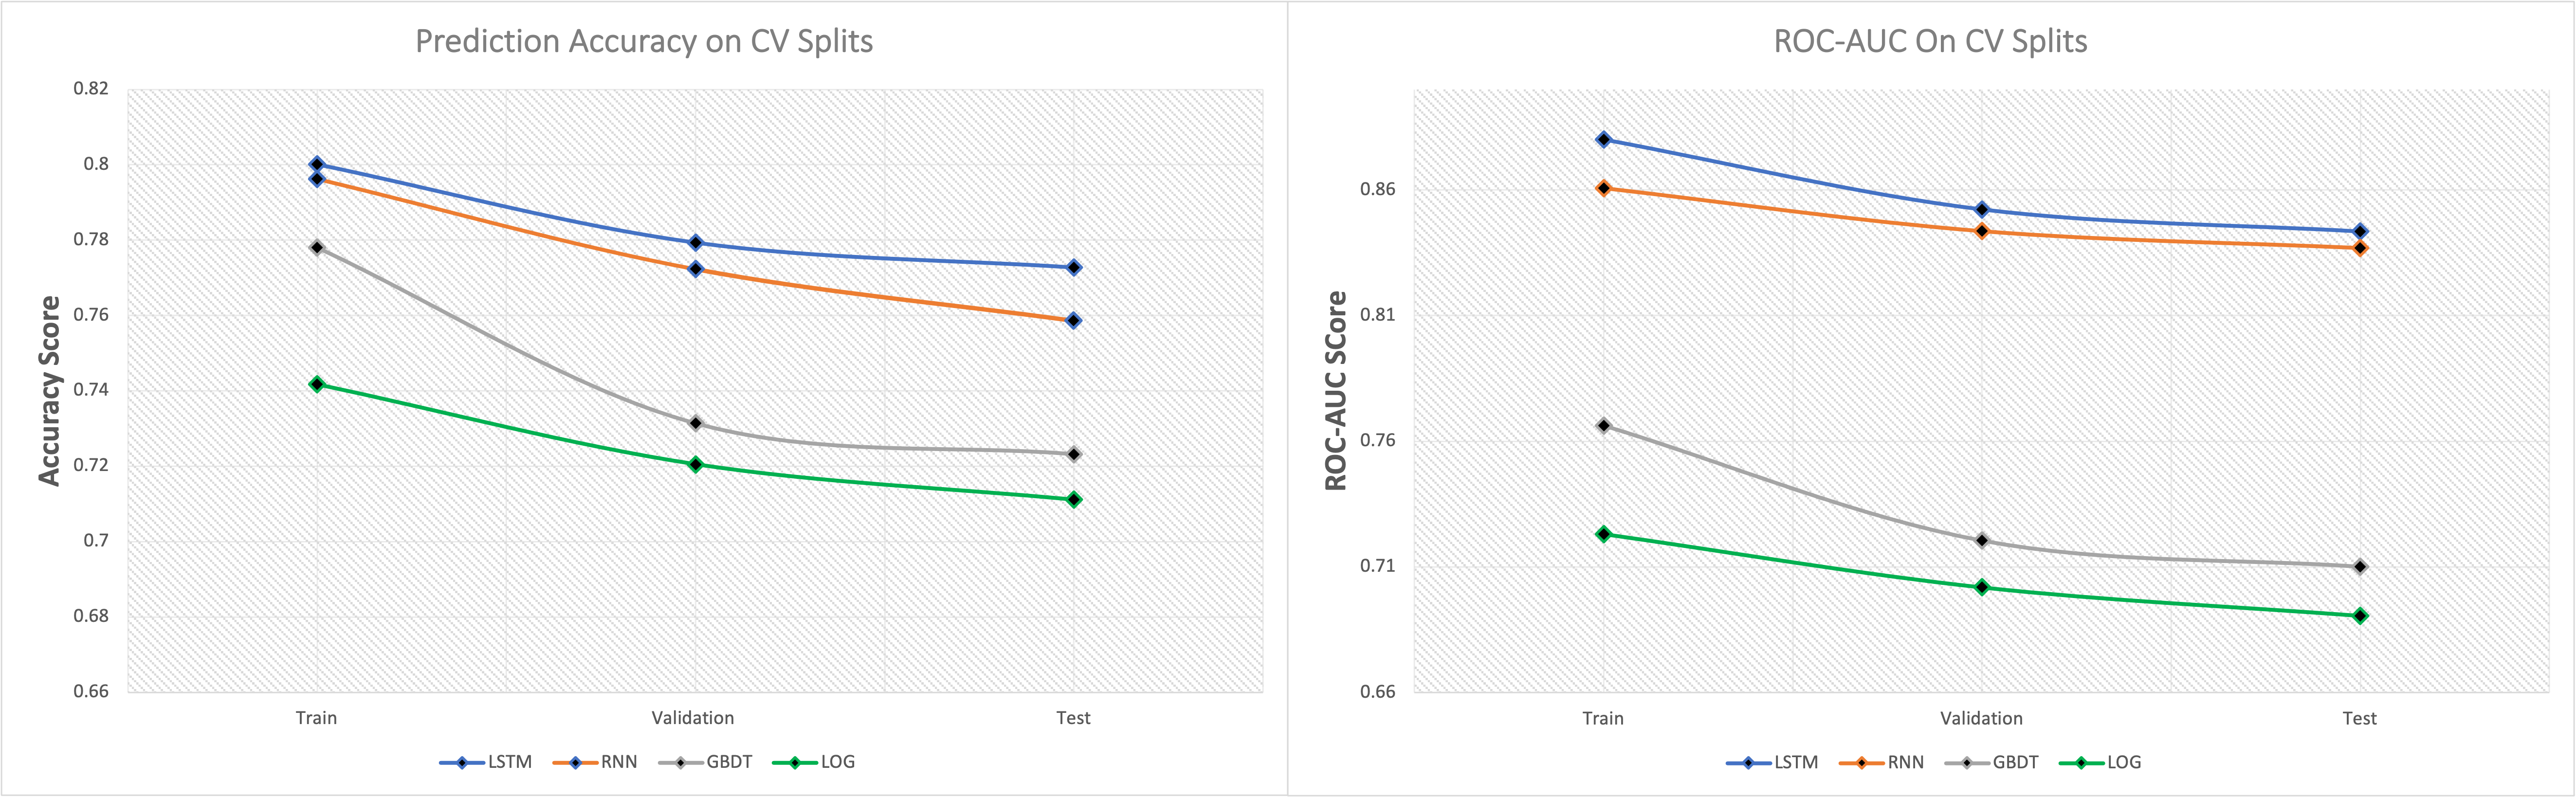
\includegraphics[width = \linewidth]{cvResults.png}
        \caption{Cross Validation Results}
        \label{fig:CV Results}
    \end{figure}
    \begin{multicols*}{2}           
    

                
    \section{Results}

        \subsection{Cross Validation Metrics}

            \paragraph{}
                The scores for accuracy and ROC-AUC over the various cross validation folds are given in Figure 10.
                Note that the models are re-trained using all prior data before the final test fold.
                Looking at the test metrics, the sequential models outperform the baselines.
                The best LSTM (accuracy 0.7727 ROC-AUC 0.8434) slightly outperforms the best RNN (accuracy 0.7586 ROC-AUC 0.8369) model.  
                This is a considerable increase over the best performing GBDT (accuracy 0.7323 ROC-AUC 0.7101) and logistic regression (accuracy 0.7111 ROC-AUC 0.6906) models. 
                The sequential approach gives around a 3-6\% accuracy boost in predicting play calls and a 12-15\% boost in the seperability of runs and passes.
                
            \vspace{-10pt}

            \paragraph{}
                Importantly, for the sequential models, the metrics stay relatively steady over the training, validation, and test folds.
                This is solid indication that these kinds of models will generalize well to data outside what is considered in this analysis (i.e. different NFL seasons).  
                There is an expected drop off in performance going from training to testing as the model hasn't seen the test data. 
                A large discrepancy between training and testing metrics is indication of the model overfitting.
                This is apparent for GBDT, where a considerable performance dropoff occurrs between training and validation/testing.
                Even though its final test metric is slightly worse, the logistic regression model may be preffered over GBDT as its metrics remain steady over the folds. 
                 
        
        \subsection{Selected Hyperparameters}

            \paragraph{}
                A list of chosen hyperparameters for the best LSTM model is given in Table 5. 
                The best performing model uses 11 previous play calls as a sequence. 
                Note this model is relatively simple with only one sequential and dense layer each.
                The amount of recurrent units (54) falls in an intermediate value, finding a good balance between overly-simplistic and overly-complex. 
                The dropout rates fall near the middle of their specified ranges as well, balancing the right amount of training information to lose in order to generalize the predictions.
                
        
        \begin{center}
        \begin{tabular}{|| m{3cm} | m{3cm}||}
            \hline
            \textbf{Parameter} & \textbf{Value}  \\
            \hline\hline
            Sequence Length & 11  \\
            \hline
            Sequential Layers & 1 \\
            \hline
            Units & 54 \\
            \hline
            Dense Layers & 1 \\
            \hline
            Dense Dropout & 0.205 \\
            \hline
            LSTM Dropout & 0.159 \\
            \hline
            Learning Rate & 0.0067\\
            \hline 
        \end{tabular}
        \captionof{table}{LSTM Hyperparameters}
        \end{center}

            \paragraph{}
                A similar table for the best selected RNN model is given in Table 6.
                Suprisingly, the RNN model considers a longer play sequence (12) than LSTM. 
                A simpler model is chosen for this type as well (only one sequential and dense layer each).
                The lower value of recurrent units (27) shows simplicity was favored even more for RNNs.   
                For the RNN and dense dropout, the values selected are closer to the bottom of the specified range. 
                This indicates the model needs all the information from the inputs in order to perform well, which is not suprising as RNNs have a more simple structure.
                The learning rates for both models are similar and relatively high, indicating that optimal models are able to converge quickly.   
        \begin{center}
            \begin{tabular}{|| m{3cm} | m{3cm}||}
                \hline
                \textbf{Parameter} & \textbf{Value}  \\
                \hline\hline
                Sequence Length & 12  \\
                \hline
                Sequential Layers & 1 \\
                \hline
                Units & 27 \\
                \hline
                Dense Layers & 1 \\
                \hline
                Dense Dropout & 0.104 \\
                \hline
                RNN Dropout & 0.135 \\
                \hline
                Rec Dropout & 0.268 \\
                \hline
                Learning Rate & 0.0058\\
                \hline
                
            \end{tabular}
            \captionof{table}{RNN Hyperparameters}
            \end{center}

            \paragraph{}
                Again, the chosen hyperparameters for the best GBDT model is show in Table 7.
                The number of estimators used was toward the larger end of the range. 
                This means the algorithm took a relatively long time to converge on a good solution.
                The regularization parameters are moderate to high for all of minimum samples per leaf, minimum sample to split, and max depth (lower values of max depth mean higher regularization).
                So, even with such high levels of regularization, the GBDT model still showed the highest degree of overfitting.  
                
        \begin{center}
            \begin{tabular}{|| m{3.25cm} | m{3cm}||}
                \hline
                \textbf{Parameter} & \textbf{Value}  \\
                \hline\hline
                Estimators & 408  \\
                \hline
                Subsample & 0.89 \\
                \hline
                Min Samples Split & 9 \\
                \hline
                Min Samples Leaf & 10 \\
                \hline
                Max Depth & 2 \\
                \hline
                
            \end{tabular}
            \captionof{table}{GBDT Hyperparameters}
            \end{center}


            \paragraph{}
                Finally, the value chosen for $L_1$ ratio in the best performing logistic regression model was 0.6103. 
                A balance between $L_1$ and $L_2$ regularization was generally favored, with a slight preference for $L_1$. 

                    
        \subsection{Model Application - Red Zone}
            \paragraph{}
                Using all play call contexts is practical for building and evaluating models. 
                However, there are many situations where the play call is obvious, and some play calls are more consequential than others.
                To truly get a sense for how useful the best selected model is, it needs to be tested in critical, game deciding situations. 
                To this end, this section aims to show performance of the best model in red zone situations. 
            
            \vspace{-10pt}

            \paragraph{}
                A play is considered to be in the red zone when the offensive team is within 20 yards or less of the opposition's goal line. 
                Converting red zone plays into touchdowns is critical for the offensive team, likewise, it is critical for the defensive team to force the offensive team into a field goal attempt.
                Also, it is not apparently obvious whether a red zone play will be a pass or a run. 
                In the entire data set, 54\% of red zone plays were passes while 46\% of red zone plays were runs. 
                So, red zone plays present a particularly useful case for the model because 1) knowing the outcome provides an especially helpful competitive advantage and 2) it is hard to tell what the outcome will be.
                
            \vspace{-10pt}

            \paragraph{}
                Due to its slight increase in performance over the best RNN model, the best LSTM from the previous section was chosen for this application.
                The model was trained on all observations occurring in weeks 1 through 12 of the NFL season.
                Then, of the original test split, observations were filtered to retain only play calls happening in the red zone. 
                This leaves 1416 red zone play calls occurring during weeks 13-17 of the NFL season. 
            
            \vspace{-10pt}

            \paragraph{}
                The model returns a 0.8166 accuracy and a 0.9074 ROC-AUC score for play calls in the red zone. 
                Given the sample wide metrics on the test set, this is an encouraging result as the model performs well in the situations that matter most. 
                Even more important situations are the later downs of red zone plays. 
                Whether the defensive team is successful on third or fourth down of a red zone play will often mean the difference between winning and losing.
                Figure 11 shows prediction accuracy and ROC-AUC score of red zone plays by down. 
                The model performs very well in the later down situations and reaches nearly 88\% accuracy on third downs. 
                Having this level of confidence in the opposition's play call in a critical third and goal situation would present a massive advantage for the defensive team. 
                As a caveat, it should be noted these metrics are slightly buoyed by the relatively small amount of observations in each set (568 1st, 464 2nd, 334 3rd, 50 4th).   


            \end{multicols*}
            \begin{figure}[ht]
                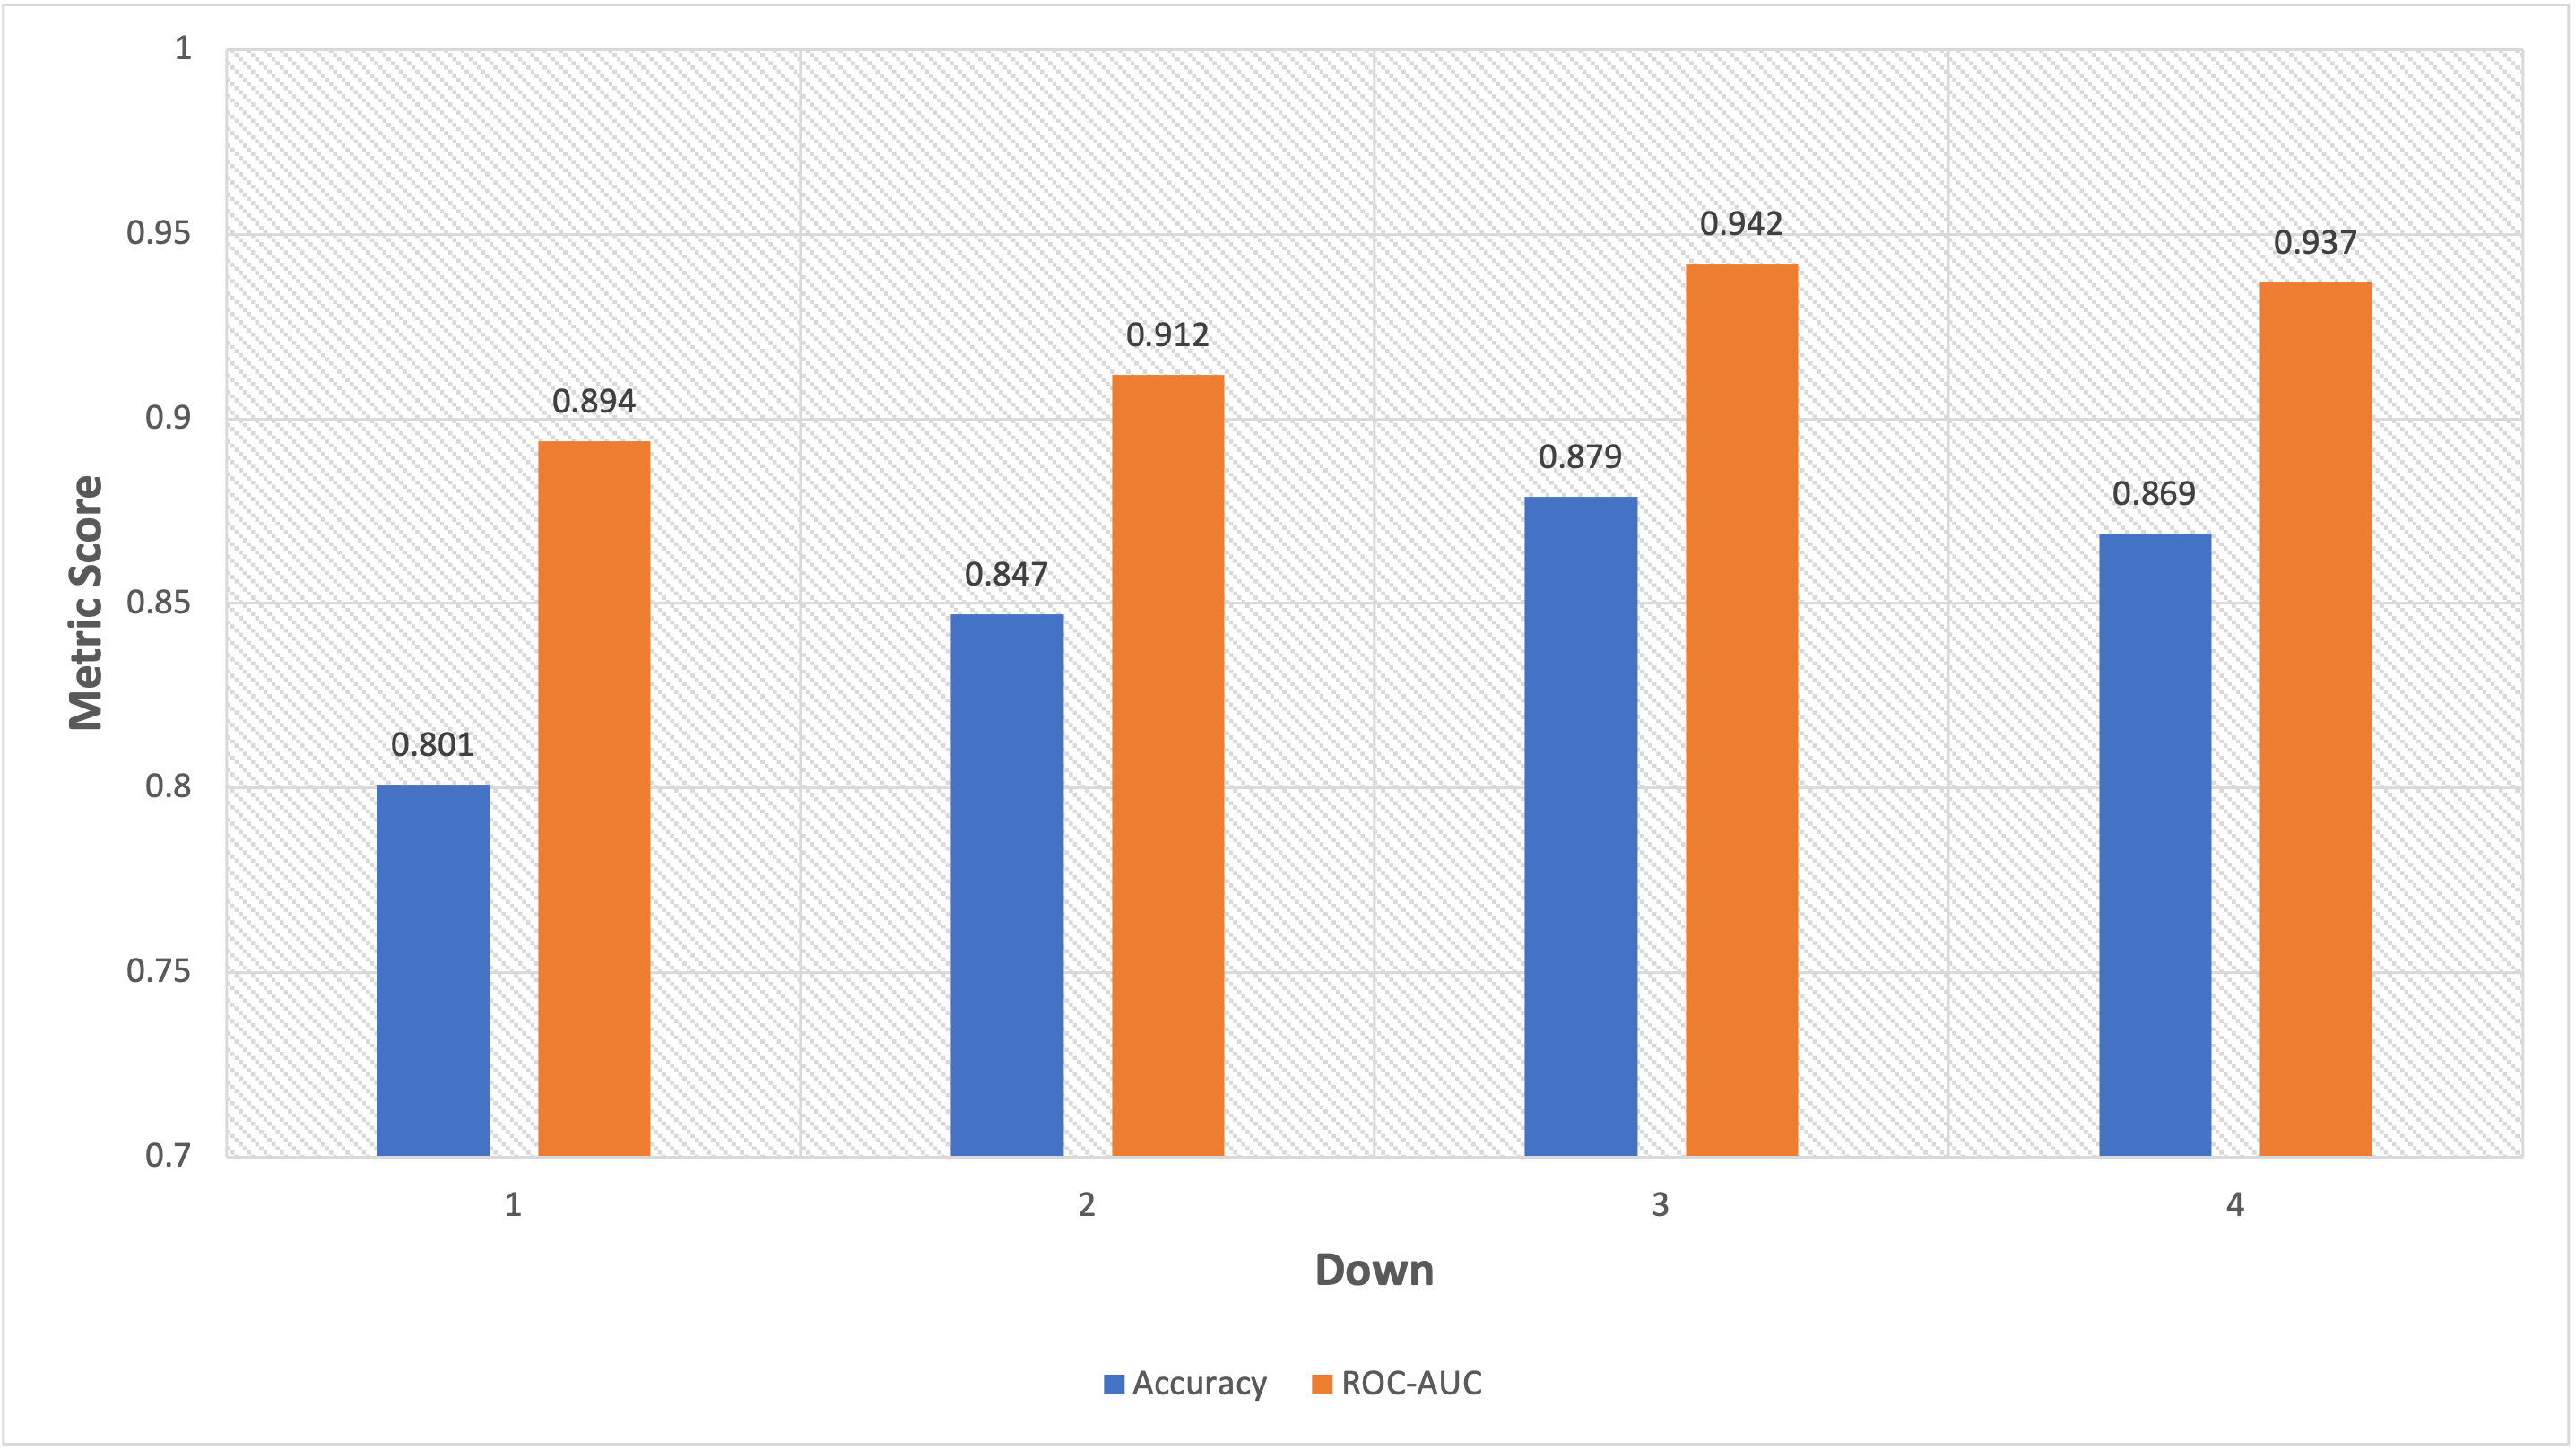
\includegraphics[width = \linewidth]{redZoneByDown.png}
                \caption{Prediction Metrics of Red Zone Plays by Down}
                \label{fig:Prediction Metrics of Red Zone Plays by Down}
            \end{figure}
            \begin{multicols*}{2} 

    \section{Discussion}

        \subsection{Takeaways}

            \paragraph{}
                As is evident by the comparative performance of models assessed in this analysis, choosing a fancier model strategy will only slightly improve results if the data is left in tabular form.  
                The performance boost from a logistic regression classifier to a gradient boosted decision tree is negligible. 
                As shown, machine learning tasks are not solved by simply throwing a more complex model at the problem. 
                Real breakthroughs come from thinking critically about the real world processes that generated the data of interest. 
                Any football fan will know that a play call is not made in an individual vacuum. 
                Hence, it is not just the current situation that influences this decision, but rather the combination of these factors and the sequence of outcomes happening beforehand.   
                
            \vspace{-10pt}
            \paragraph{}
                With this in mind, it was not the desire to use deep learning that motivated the choice of modeling strategy in this analysis, but rather a reassessment of how to structure the data. 
                Given that the idea was to structure the data as a sequential pattern, the choice of models to use simply followed from what has been proven to work with data in this form. 
                The results prove this was an effective strategy and confirm the presence of a temporal component in NFL play calls.
                
            \vspace{-10pt}
            \paragraph{}
                An interesting takeaway is the optimal number of plays to consider as a sequence. 
                This aspect was able to be considered as a hyperparameter of the sequential models. 
                Going into the analysis it was anticipated this value would only be up to the 4 or 5 most recent plays.
                To the contrary, many of the best performing sequential models happened to consider play call histories of over 10 plays. 
                This challenged the preconceived notion of what a play call sequence would look like. 
                10 plays is around the average amount an offensive team will run on a sustained scoring drive. 
                It makes sense that the model would need the entire history of a drive to predict accurately, as it would be able to store information at every stage. 


            \vspace{-10pt}
            \paragraph{}
                Overall, simpler models were favored in this analysis.
                While there is enough of a performance boost using sequential models to show there is a temporal pattern to the data, this relationship isn't complex enough to warrant the use of multiple hidden recurrent layers.
                This is an encouraging sign as simple models are easier to construct and take less computational resources to train.
        

        \subsection{Limitations}
            \paragraph{}
                A general challenge with modeling this data is that it is designed to be deceptive. 
                The offensive team survives off of tricking the defense and is fully aware of its own tendencies. 
                It knows what it is expected to do at any given situation and will often do the exact opposite in order to maintain an element of surprise. 
                Due to this nature, it seems there will always be a less than desirable upper limit on model performance no matter how much quality data is fed into an algorithm.

            \vspace{-10pt}
            \paragraph{}
                Another significant limitation to the results of this analysis is the lack of quality data.
                Two massively critical aspects to determining play calls are not included in the feature space.
                These factors are the specific formation that offense lines up in and the personnel packages on the field for the current play. 
                Due to not knowing these details, any model's performance is greatly reduced because there is valuable information influencing the response that it can't account for. 
                In particular, knowing the formation and personnel would help the model distinguish classes in situations where the play call isn't obvious. 
                An example would be first and long situations where the frequency of passes and runs is nearly even. 
                Most of the time this is a case where the in game context gives little to no signal. 
                Knowing whether the offense lines up in bunch formation, with two tight ends and a full back, versus the spread with five wide receivers would allow the classes to be much easier to seperate.

            \vspace{-10pt}
            \paragraph{}
                Further improving the data is the clearest path forward to build upon these results. 
                While not freely available, it does appear that some paid services (designed for Fantasy Football modeling) allow access to personnel/formation data.
                Exploring these options and attempting a similar modeling strategy as in this analysis would be worthwhile.
                In addition, simply adding more data from multiple NFL seasons could somewhat improve results. 
                This analysis focused on one season alone in order to use the teams as features. 
                Since teams can even change over the course of a single season (injuries, trades, etc.), the assumption that they remain constant may be invalid.
                A suggestion would be to not consider offensive or defensive team as a feature in the model and use many years of data for training/testing.  


\newpage
\end{multicols*}
\begin{thebibliography}{999}

    \bibitem{Mehryar12}
        Mehryar Mohri, Afshin Rostamizadeh, Ameet Talwalkar.
      \emph{Foundations of Machine Learning}.
      The MIT Press,
      2012.
      
    \bibitem{Haykin08}
      Haykin
    \emph{Neural Networks and Learning Machines}.
    Pearson, 3rd Edition,
    2008.

    \bibitem{Li15}
    X. Li and X. Wu. (2015)
    \emph{Constructing Long Short-Term Memory based Deep Recurrent Neural Networks for Large Vocabulary Speech Recognition}.
    IEEE International Conference on Acoustics, Speech and Signal Processing

    \bibitem{Patel20}
    Patel, P. (2020). Retrieved April 21, 2022, from https://sites.northwestern.edu/msia/2020/01/31/nfl-tendency-analysis-and-basic-play-type-prediction/. 

    \bibitem{Carl22}
    Carl S, Baldwin B (2022). \emph{nflfastR: Functions to Efficiently Access NFL Play by Play Data}. https://www.nflfastr.com/, https://github.com/nflverse/nflfastR.

    \bibitem{Brownlee20}
    Brownlee, Jason. (2020). \emph{Ordinal and One-Hot Encodings for Categorical Data}. Machinelearningmastery. https://machinelearningmastery.com/one-hot-encoding-for-categorical-data//
    
    \bibitem{Dupond19}
    Dupond, Samuel (2019). \emph{A thorough review on the current advance of neural network structures}. Annual Reviews in Control.

    \bibitem{Murilo22}
    Gustineli, Murilo (2022). \emph{A survey on recently proposed activation functions for Deep Learning}. arXiv:2204.02921

    \bibitem{Mozer95}
    Mozer, M. C. (1995). \emph{A Focused Backpropagation Algorithm for Temporal Pattern Recognition}. In Chauvin, Y.; Rumelhart, D. (eds.). Backpropagation: Theory, architectures, and applications. ResearchGate. Hillsdale, NJ: Lawrence Erlbaum Associates.

    \bibitem{Olah15}
    Olah, C. (2015). \emph{Understanding LSTM Networks}. Retrieved April 21, 2022, from https://colah.github.io/posts/2015-08-Understanding-LSTMs//.
    
    \bibitem{Hastie01}
    Hastie, T., Hastie, T., Tibshirani, R., Friedman, J. H. (2001). \emph{The elements of statistical learning: Data mining, inference, and prediction}. New York: Springer.

    \bibitem{Jameison17}
    Li, L., Jamieson, K., DeSalvo, G., Rostamizadeh, A., Talwalkar, A. (2017). \emph{Hyperband: A novel bandit-based approach to hyperparameter optimization}. The Journal of Machine Learning Research, 18(1), 6765-6816.
    
\end{thebibliography}
\end{document}